\documentclass[UTF8,nofonts]{ctexart}
\date{\today}
\usepackage{geometry}
\usepackage{fancyhdr}
\usepackage{amsmath}
\usepackage{algorithm2e}
\usepackage{graphicx}
\setCJKmainfont{微软雅黑}
\setmainfont{微软雅黑}
\linespread{1.6}
\geometry{a4paper,left=3cm,right=3cm,bottom=3cm}
\pagestyle{fancy}
\fancyhf{}
\rfoot{\thepage}
\lhead{ }
\renewcommand\headrulewidth{0.8pt}
\begin{document}
\newpage
\vspace{1cm}
\section{Principles of Neural Science:Memory}
在加西亚.马尔克斯的著名作品百年孤独中,描述了这样的一种奇怪的瘟疫。这个瘟疫袭击了一个小村庄,染上瘟疫的人会逐渐的丧失记忆:首先是个人的过往记忆,然后是常见器物的名字和用途。一个人为了与这种瘟疫做斗争,在自己家的所有器物上都贴上便笺。但是随着词语和字母的认知能力的丧失,一切抗争都归为徒劳。
\par
这段离奇故事从某个角度上说明了学习和记忆在我们日常生活中的作用。学习指的是通过获得的知识来改变行为,而记忆指的是我们对这些知识的编码、存储以及检索的过程。在1861年Broca发现左额叶的后部(Broca区)损伤会导致语言功能的退化,这个发现引发了脑功能区的划分热潮。脑功能区的离散划分自然而然的引发了下面这个问题:这些功能区是不是通过记忆相连的呢?如果真的是通过记忆相连的话,记忆是通过一个记忆中心相连呢还是广泛的分布于各脑区?
\par
过去的几十年中,学习和记忆方面的研究有了很大的进展。当前章节中,我们将注重于下面三个方面的介绍:
\begin{enumerate}
\item 学习和记忆有很多类型,不同的类型有不同的认知性质,由不同的脑区控制。
\item 记忆可以分解为编码、存储强化、检索这三个过程。
\item 记忆的相关异常可以为学习和记忆的研究提供线索。
\end{enumerate}
记忆能够分解为两个维度:时间维度和存储结构。我们这里首先来探讨一下时间维度。
\subsection{长期记忆和短期记忆牵涉到不同的神经系统}
\subsubsection{短期记忆维持当前目标相关信息的呈现}
当提到记忆的时候,我们一般想起的是长期记忆,而忽视了短期记忆。但是,长期记忆是由短期记忆固化而来的。短期记忆,也叫做\textit{working memory},维持着容易消失的当前目标相关知识的呈现。人类的\textit{work memory}至少包含两个子系统:一个与语言(verbal)相关,一个与视觉(visuospatial)相关。这两个子系统由第三个子系统--\textit{executive control process} 调控。这个\textit{executive control process} 的主要功能是分配注意力,监控、操控及更新所存储的知识表达。
\par
语言子系统又包括两个子系统:一个用来存储语音相关的知识,一个用来回响接收的语音输入。神经生理学和神经成像的数据表明:语音知识的存储与后顶叶皮层有关,而回响则需要Broca区的参与。
\par
视觉子系统又与顶叶、内测颞叶、枕骨外皮层、前额叶、运动前皮层相关。至于这个视觉子系统是否可以分解为空间和物体这两个子系统,人们目前还没有定论。
\subsubsection{短期记忆会被选择性的转换为长期记忆}
在1950年代,学界从癫痫病人的切除治疗中获得了长期记忆是从短期记忆转换而来的惊人证据。这些病人的中颞叶的双侧海马和附近区域都被切除了,由此造成了这些病人的长期记忆形成障碍。这些病人中,最出名的就是代号为H.M.(为了维护病人隐私)的病人,心理学家Brenda Milner和外科医师William Scoville对这个病人做了长期的观察。2008-12-1,H.M.去世,他的真实姓名Henry Molaison才被披露出来。
\par
当时,病人H.M.为27岁的男性,7岁时由于自行车事故引起了脑部损伤,并因此忍受了10多年的不可治疗的颞叶癫痫。Scoville移除了这个病人的海马组织、杏仁核和双侧颞叶的multimodal association 区。在这个手术之后,H.M.的癫痫得到了很好的控制,但是他的记忆却损伤很大。但是,HM的记忆损伤非常特别,这种情况引起了人们的注意。
\par
HM仍然有正常的短期记忆(working memory),从几秒到几分钟不等。这个症状说明,中颞叶对于短期记忆来说并不是必须的。此外,HM对于手术之前的长期记忆仍然保持的很好。HM现在最主要的记忆困难是无法将新的短期记忆转换为长期记忆。他无法在记忆中维持刚刚认识的人、刚刚经历过的事情这些信息。当被要求背诵一个电话号码的时候,HM在几分钟之内仍然能够很好的完成这项任务。但是一旦将他的注意力转移,HM则会丧失对这个电话号码的记忆。HM并不是一个孤立的现象,所有经历过广泛双侧中间颞叶切除的病人都或多或少的会有短期记忆无法转换到长期记忆的症状。
\par
HM的重要性在于,他的功能损伤是证明记忆与中间颞叶(包括海马体)有关的第一个有效证据。考虑到海马体的大小比较大,人们不禁想知道:到底多大的损伤才会导致长期记忆困难?另外一个病人RB的临床病例表明,即使海马体只受损了一小部分,长期记忆仍然会受到很大的损伤。不同部位的损伤造成的后果可能不一样,例如海马体下面的前内鼻区(perirhinal)皮层损伤对于物体识别的影响比海马体上面的皮层损伤所造成的影响大。一些学者认为,海马体在空间认知方面的重要性比物体识别的重要性大得多。在人类身上的脑功能成像实验表明:右侧海马在涉及到空间信息记忆的行为中活动增强,而左侧海马在涉及到文字、物体及人物识别行为中活动增强。这个结论与临床上相关区域受损病人的症状相吻合。
\subsubsection{长期记忆可以分为显式记忆和隐式记忆}
在病人HM身上还观察到另外一个症状:并不是所有类型的长期记忆都完全受损,有些类型的长期记忆甚至是完全正常的。经历过类似手术病人大多也有这种症状。这种未受损的长期记忆大都来自于反射学习:即长期的重复某些活动从而得到了这个活动的长期记忆。比较生动形象的例子就是学自行车。但是反射学习并不仅仅限制在运动学习这一块,还包括habituation ,sensitization ,classical conditioning and operant conditioning。这类反射学习相关的记忆叫做隐式记忆(nondeclarative or procedural memory),这类记忆的检索完完全全是在意识无关的状态下进行的。而另外一种需要在意识作用下检索的记忆叫做显式记忆(declarative memory),它主要包括对于人、物和地点的事实知识。显式记忆是非常灵活的,多种不同环境的记忆片段可以一起链接起来。而隐式记忆则限制在特定场景下才能触发,也就是当时学习的环境条件。
\subsubsection{显式记忆拥有片段及语义形式}
加拿大心理学家Endel Tulving第一次提出了下面的观点:显示记忆可以被分类为两类-片段记忆(episodic memory)和语义(semantic)记忆。场景记忆是用来存储个人经历相关的知识,而语义记忆则是用来存储词汇和概念的意义。
\begin{figure}[h]
\centering
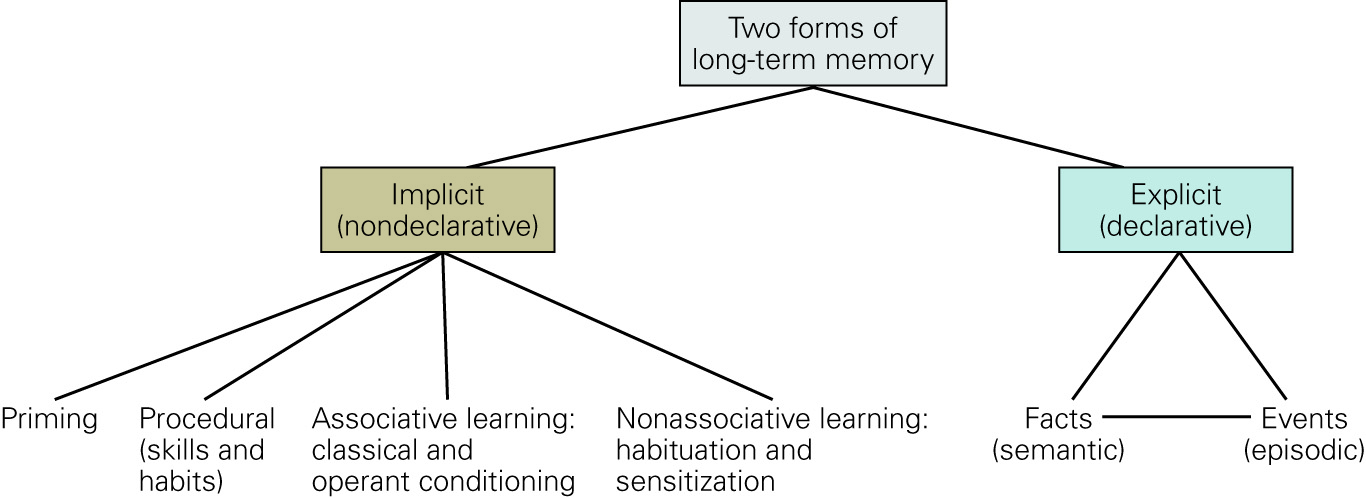
\includegraphics{Pic/6505_PNS5.jpg}
\end{figure}
对于显式记忆,我们还有如下的认识。
\begin{enumerate}
\item 大脑并没有一个单一的长期的显式记忆存储,而是分布在大脑的各个部分。这些不同部分的记忆检索可以被不同的方式独立触发,例如视觉、语音以及其他的感官信息。
\item 显式记忆至少有四个不同的信息处理过程: 编码(encoding),存储(storage),强化(consolidation),检索(retrieval)。这里我就不详细说了。
\end{enumerate}
\subsubsection{场景记忆依赖于中颞叶与相关皮层的交互}
临床失忆症病例表明,中颞叶的受损会影响在记忆上的所有四种操作:编码,存储,强化,检索,很难按照区域对功能进行定位。在PET和fMRI的帮助下,我们才能具体的观察各个不同区域在不同操作下的影响。fMRI表明:在涉及到深度编码(例如判断一个单词是具体还是抽象)时中颞叶的活动比浅显编码(例如是否一个单词是大写的还是小写的)时活动更强。左前额叶皮层在深度编码时,活动也会增强。这些证据表明前额叶与中颞叶在编码场景记忆是有很大的作用。后续的实验表明:场景记忆依赖于前额叶的认知控制过程和中颞叶的关联绑定机制之间的交互。
\par
中颞叶的不同的皮质区之间的交互对于记忆强化这个过程非常重要。HM的事例表明,老的记忆并不存储在中颞叶这里。根据Larry Squire等人的相关研究,中颞叶在记忆强化过程中只是当作一个临时存储区,这个存储区所存储的记忆会随着时间而衰退,而这些衰退的记忆会转移到皮质区。当记忆检索的时候,会同时检索这两个区域。失忆病人的症状与这个推论相吻合。
\par
\subsubsection{语义知识存储在不同的关联皮层以及检索依赖于前额页}
语义知识是我们对于这个世界的认识:包括客观事实、概念,以及词汇的意义。语义知识与场景知识的不同之处在于:语义知识与学习该知识所在的上下文无关。语义知识分布式的存储在大脑皮层中,包括颞叶的外侧和腹侧。不同的存储区域存储不同的信息,受损伤时只会影响特定的语义知识。Rosaleen McCarthy和Elizabeth Warrington 观察到拥有以下症状的病人:对于有生命的物体的知识受损,但是对于无生命的物体的知识保存完好。例如,一个病人把毛巾描述为“可以用来擦干身体的物体”,而把黄蜂描述为“一种会飞的鸟”。其他病人有刚好相反的症状。这些例子表明大脑是以概念原语来存储知识的,即 概念图谱。使用PET和fMRI的神经成像实验表明在正常人的大脑中知识是按照不同类别管理的。当人们被要求描述在照片中的动物时,左内侧颞叶活动增强。当被要求描述照片中的工具时,左前运动区和左中颞叶活动增强,这两个区域分别管理
使用物体时人运动的形式以及物体自己的运动形式。
\subsubsection{隐式记忆支持知觉启动(Perceptual Priming)}
隐式记忆存储那些下意识得到的知识。Priming是一种并不依赖于中颞叶的隐式记忆,在失忆症病人和正常人群中都有这种记忆。当前人们提出两种priming:\textit{Conceptual priming}和\textit{Perceptual priming}。Conceptual priming 提供任务相关的语义知识的快速访问,因为这些知识已经使用过了。而perceptual priming 则与具体的感觉信息有关。根据Tulving 和Schater ,perceptual priming 依赖于管理词语、对象的形式和结构感觉信息的皮质区。
对于皮层单一感觉区域的损伤会印象到该感觉调节相关的perceptual priming 。例如,右枕区广泛病变的病人无法正确处理词语的视觉priming,但是拥有正常的显式记忆。这个病例与HM刚好相反,说明priming的机制与显式记忆的机制是不同的。
\par
视觉priming总是伴随着高级视觉中枢的活动减弱。Randy Buckner 及其同事通过fMRI发现带外皮层(extrastriate cortex)的第一次打看到物体时的活动水平比之后看到同样物体的活动水平更高。这个发现也佐证了另外一个发现:左前额皮层的活动在概念priming时是减弱的。
\par
另外的一种隐式记忆是与学习相关的记忆,包括运动学习、感知学习以及习惯学习。运动学习这类记忆是通过重复的运动来得到的。这类运动感觉技巧的学习牵涉到基底节、小脑以及大脑皮层。帕金森与亨廷顿病人的基底节受损,从而无法学习运动技巧。小脑损伤也会造成类似后果。最后,熟练的运动行为都需要在相关的脑区的结构变化来得到固化,例如音乐家的手指部分。
\par
感知学习可以提高利用感官信息的能力,例如读取镜子中的逆向文本。通过不断的练习读取逆向文本,相关活动牵涉到的功能区也会发生改变。该开始的时候,读取活动会引起腹侧视觉处理区一级顶部皮层的活动增强。但是随着训练的进行,顶部皮层活动开始减弱,而左内侧颞皮层的活动开始增强。这个区域主要与视觉的表现形式有关,说明不断地练习读取逆向文本会把将文本逆转这个步骤消除,而直接从逆转文本中反射得到正向文本。即,相关的感觉学习从认知参与到自主反射的转变,所谓的习惯成自然。
\subsubsection{隐式记忆既可以是关联的也可以是非关联的}
所谓的关联记忆,指的是不同刺激之间或者刺激与行为之间的联系。而所谓的非关联记忆,指的是单个刺激的属性。非关联学习主要牵涉到单一刺激的长期作用,其结果主要有两类:习惯化(habituation)和敏感化(sensitization)。这两个词的意思很直接,这里就不再做多解释。在这两种情境下,刺激出现的时间并不重要。而在关联记忆中,两个刺激之间的先后关系很大程度的影响了关联记忆的强度。经典的条件发射牵涉到学习两个不同刺激之间的关系,而操作条件发射(operant conditioning)则涉及到学习一个行为的后果。
\subsubsection{经典条件反射牵涉到两个刺激之间的关联}
经典条件发射的喜闻乐见的例子就是驯狗大师巴普洛夫了。这个故事也是老生常谈,这里略去不提。这个经典条件发射牵涉到两个刺激:条件刺激(conditioned stimulus)和非条件刺激(unconditioned stimulus)。重复的条件刺激伴随着非条件刺激会引起脑对条件刺激的期望,也就是频发模式挖掘(frequent pattern mining)。这个关联确立之后,并不是永久的,如果多次非条件刺激缺失则会造成关联的extinction。更多的研究发现,这两个刺激的先后顺序并不重要,重要的是这两个刺激的时间间隔。
\par
脑的多个区域与关联学习有关。吹眼睛实验表明:大脑蚁(vermis)的损伤会导致条件刺激的无效化,但并不影响非条件刺激。
\subsubsection{操作条件反射牵涉到具体行为及其后果的强化}
所谓的操作条件发射比较通俗的说法就是尝试(trail and error) ,也就是对于具体行为的评价和反馈。人们普遍认为,虽然这两种反射的分型很明显,但是其底层机制应该是差不多的。越是与生存行为相关的刺激,大脑对这个刺激的记忆越强烈。其中最明显的就是味觉厌恶(taste aversion)。即使味觉条件刺激与呕吐相差的时间超过一小时,这两者的关联仍然很紧密。但是如果是视觉或者听觉刺激伴随着呕吐,则这两者的记忆关联则不是很强。即生物体并没有所谓的auditory aversion 和visual aversion。
\subsubsection{记忆相关的疾病和缺陷给予我们更多对于正常记忆的认识}
Daniel Schacter 把记忆相关的缺陷分为七类:transience ,absent-mindness ,blocking ,misattribution,suggestibility ,bias,persistence。这些单词的意思很直接,这里就不做太多解释。
\newpage
\subsection{隐式记忆存储的机制}
全书我们都在强调:所有的行为都是大脑作用下的结果,不管是正常还是不正常的大脑(所谓的行为学派)。我们所做的行为依赖于经验,而经验就是所存储的记忆。这些记忆从何而来,又是如何存储的。在本章,我们将尝试对隐式记忆的细胞和分子机制做相关介绍。
\begin{figure}[h]
	\centering
	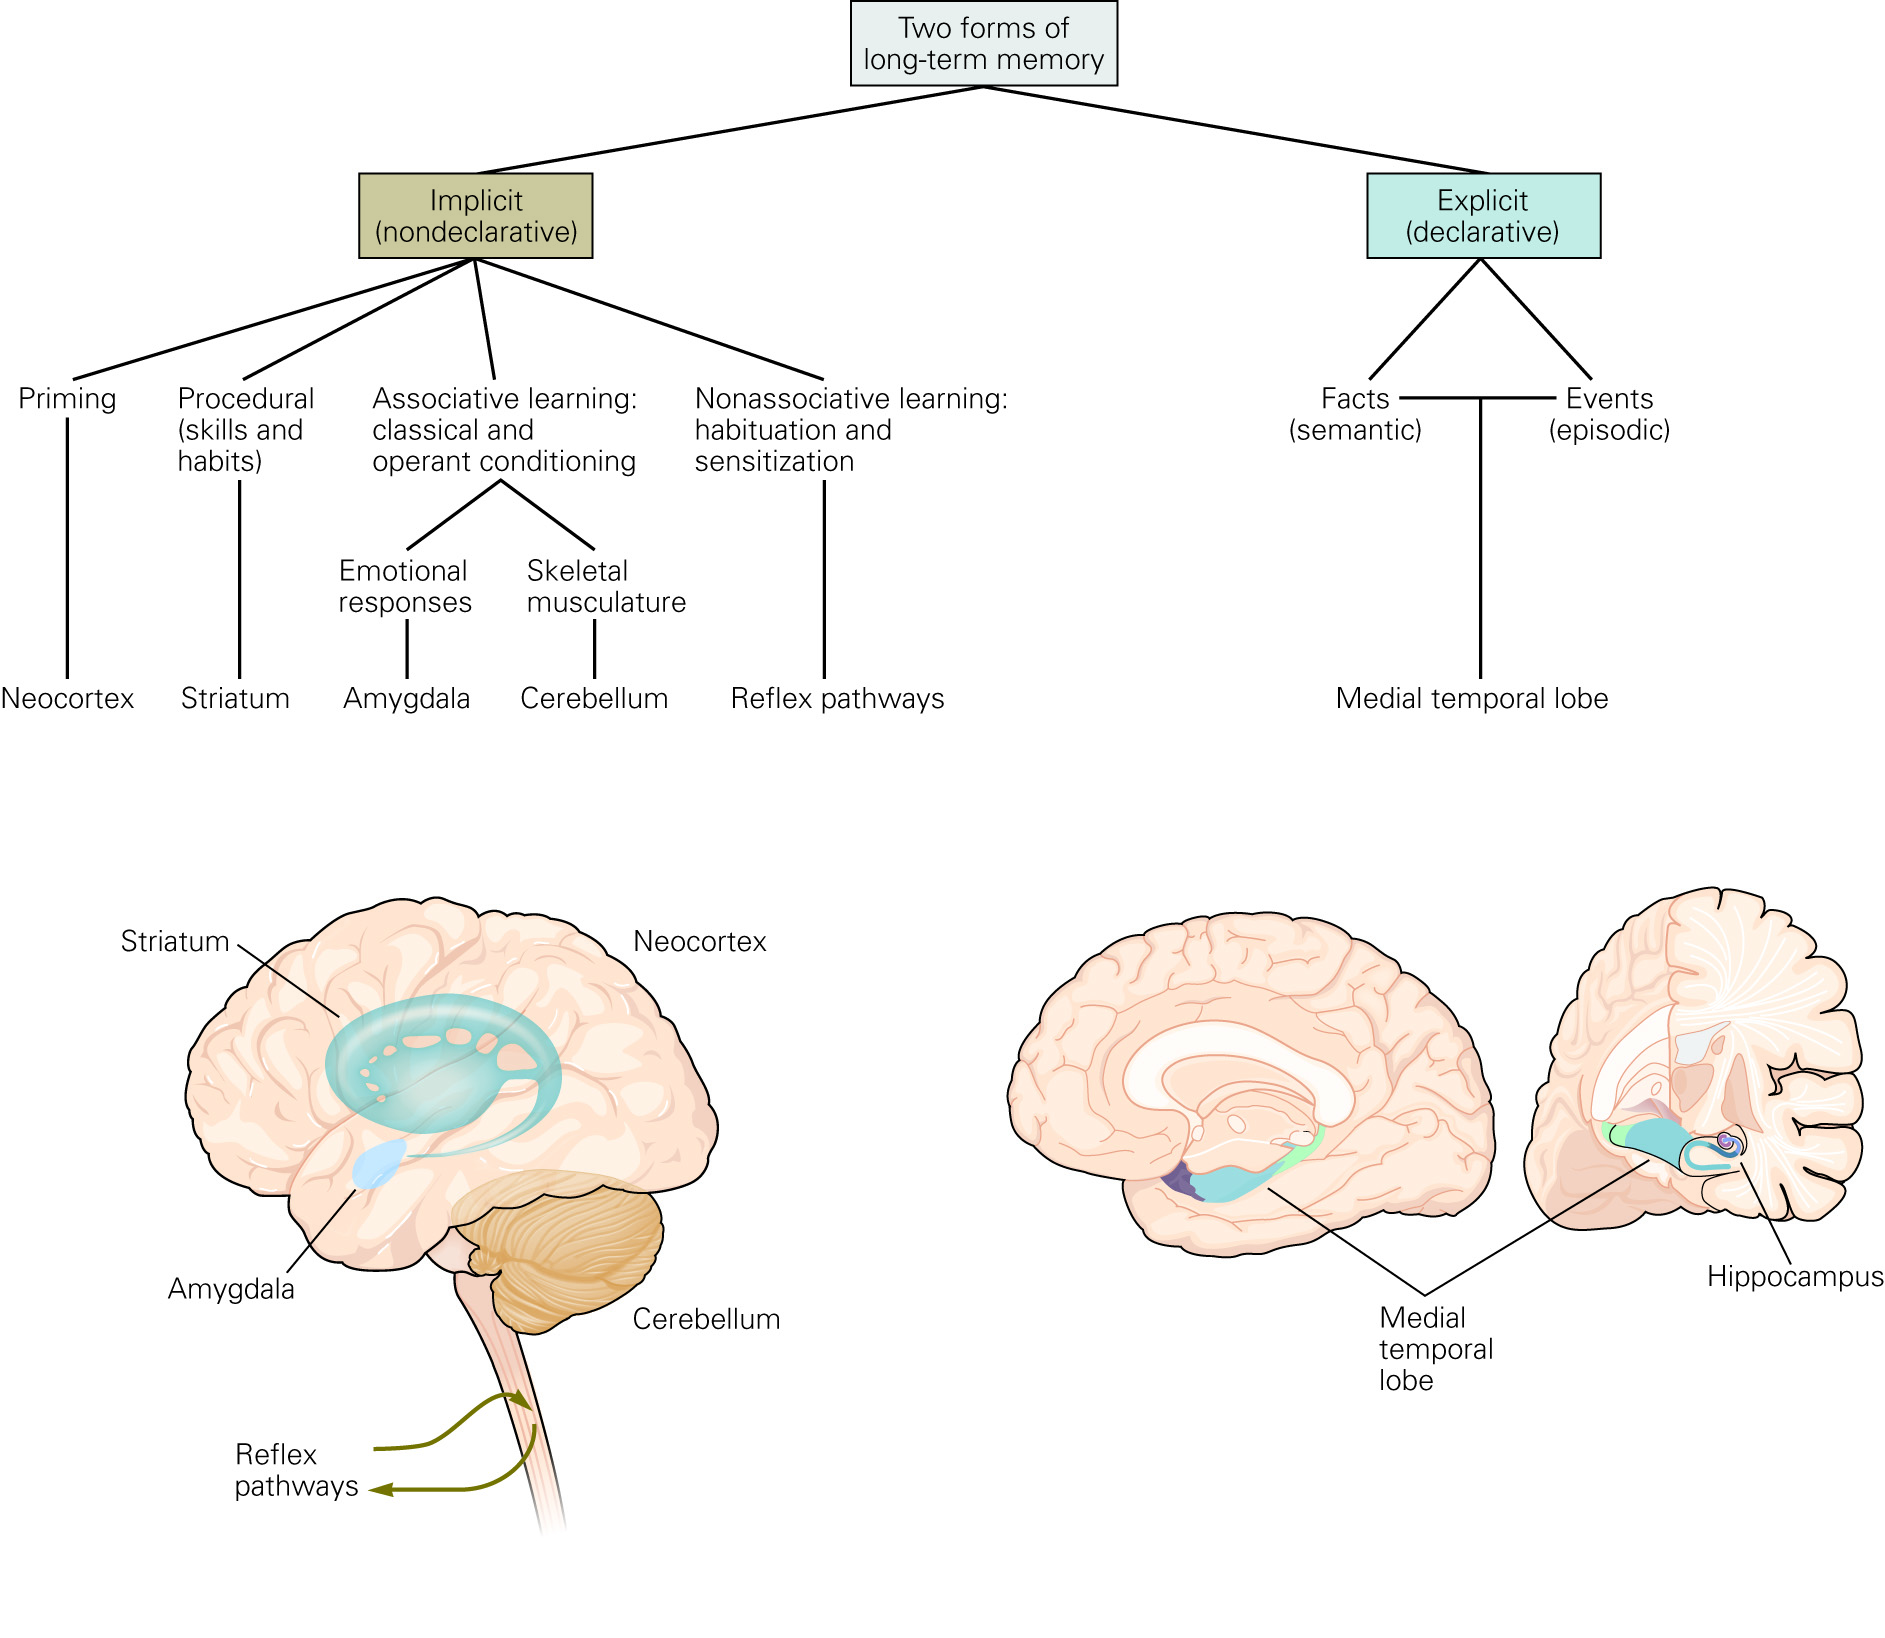
\includegraphics[scale=0.8]{Pic/6601_PNS5.jpg}
\end{figure}
\subsubsection{隐式记忆的存储与突触传输的效率相关}
在habituation,sensitization以及经典条件发射等隐式学习方面的研究提供了记忆存储基本机制的基础资料。这些学习在无脊椎动物和脊椎动物身上已经做了很详尽的研究,例如屈曲反射,恐惧应答以及眨眼。这些简单反射的学习会造成相应突触通路的效率改变。
\subsubsection{习惯化是突触传输中活动相关的突触前膜的抑制}
习惯化是最简单的一类隐式学习,它的生理学机制是被Charles Sherrington揭露的,当时他在研究猫的姿态和位置觉。Charles 观察到在重复的电刺激下,相应的反射应答的强度会减弱,他将这个现象称作 habituation。之后Alder Spencer和Richard Thomson 研究了这个现象的细胞机制。他们发现,在habituation期间,刺激部位局部的激动性中间神经元给予运动神经元的刺激会减弱。而感觉神经元与中间神经元之间的刺激强度保持不变。
\par
由于脊椎生物的中间神经元的构成非常复杂,很难分析其中的细胞机制。而海蜗牛(aplysia californica) ,由于其只有20000多个中央神经元的简单神经系统,被当作记忆研究的典型实验动物。海蜗牛有一个类似于屈曲反射的发射,而且这个反射的神经通路已经被细致的研究过了。通过触碰海蜗牛的肢体会触发机械门受体,从而引起感觉神经元的激动。感觉神经元的突触则释放出谷氨酸(glutamate),并引起中间神经元和运动细胞的快速的突触后动作电位(excitatory postsynaptic potentials),简称为EPSP。这些感觉细胞和中间神经元所产生的EPSPs在不同的时间和位置对运动细胞起作用,造成一个很强的刺激电流,并最终导致海蜗牛的快速应答。如果重复的进行刺激,由感觉神经元引起的中间神经元和运动细胞的单突触EPSP会逐渐减弱。此外,重复的刺激还会导致中间神经元与运动细胞突触间递质传输的减慢。这些因素,最终导致了反应应答的衰减。
\par
量化分析表明,在这个habituation的过程中,感觉神经元的突触前膜所分泌的谷氨酸数量会减少。谷氨酸的数量减少造成了突触小泡的数量减少,但是同时突触后膜对于谷氨酸的活性不变。由于这个过程并不涉及到其他细胞,所以这种衰减也被成为单突触抑制(homosynaptic depression)。这个抑制会持续好几分钟。
\begin{figure}[h]
	\centering
	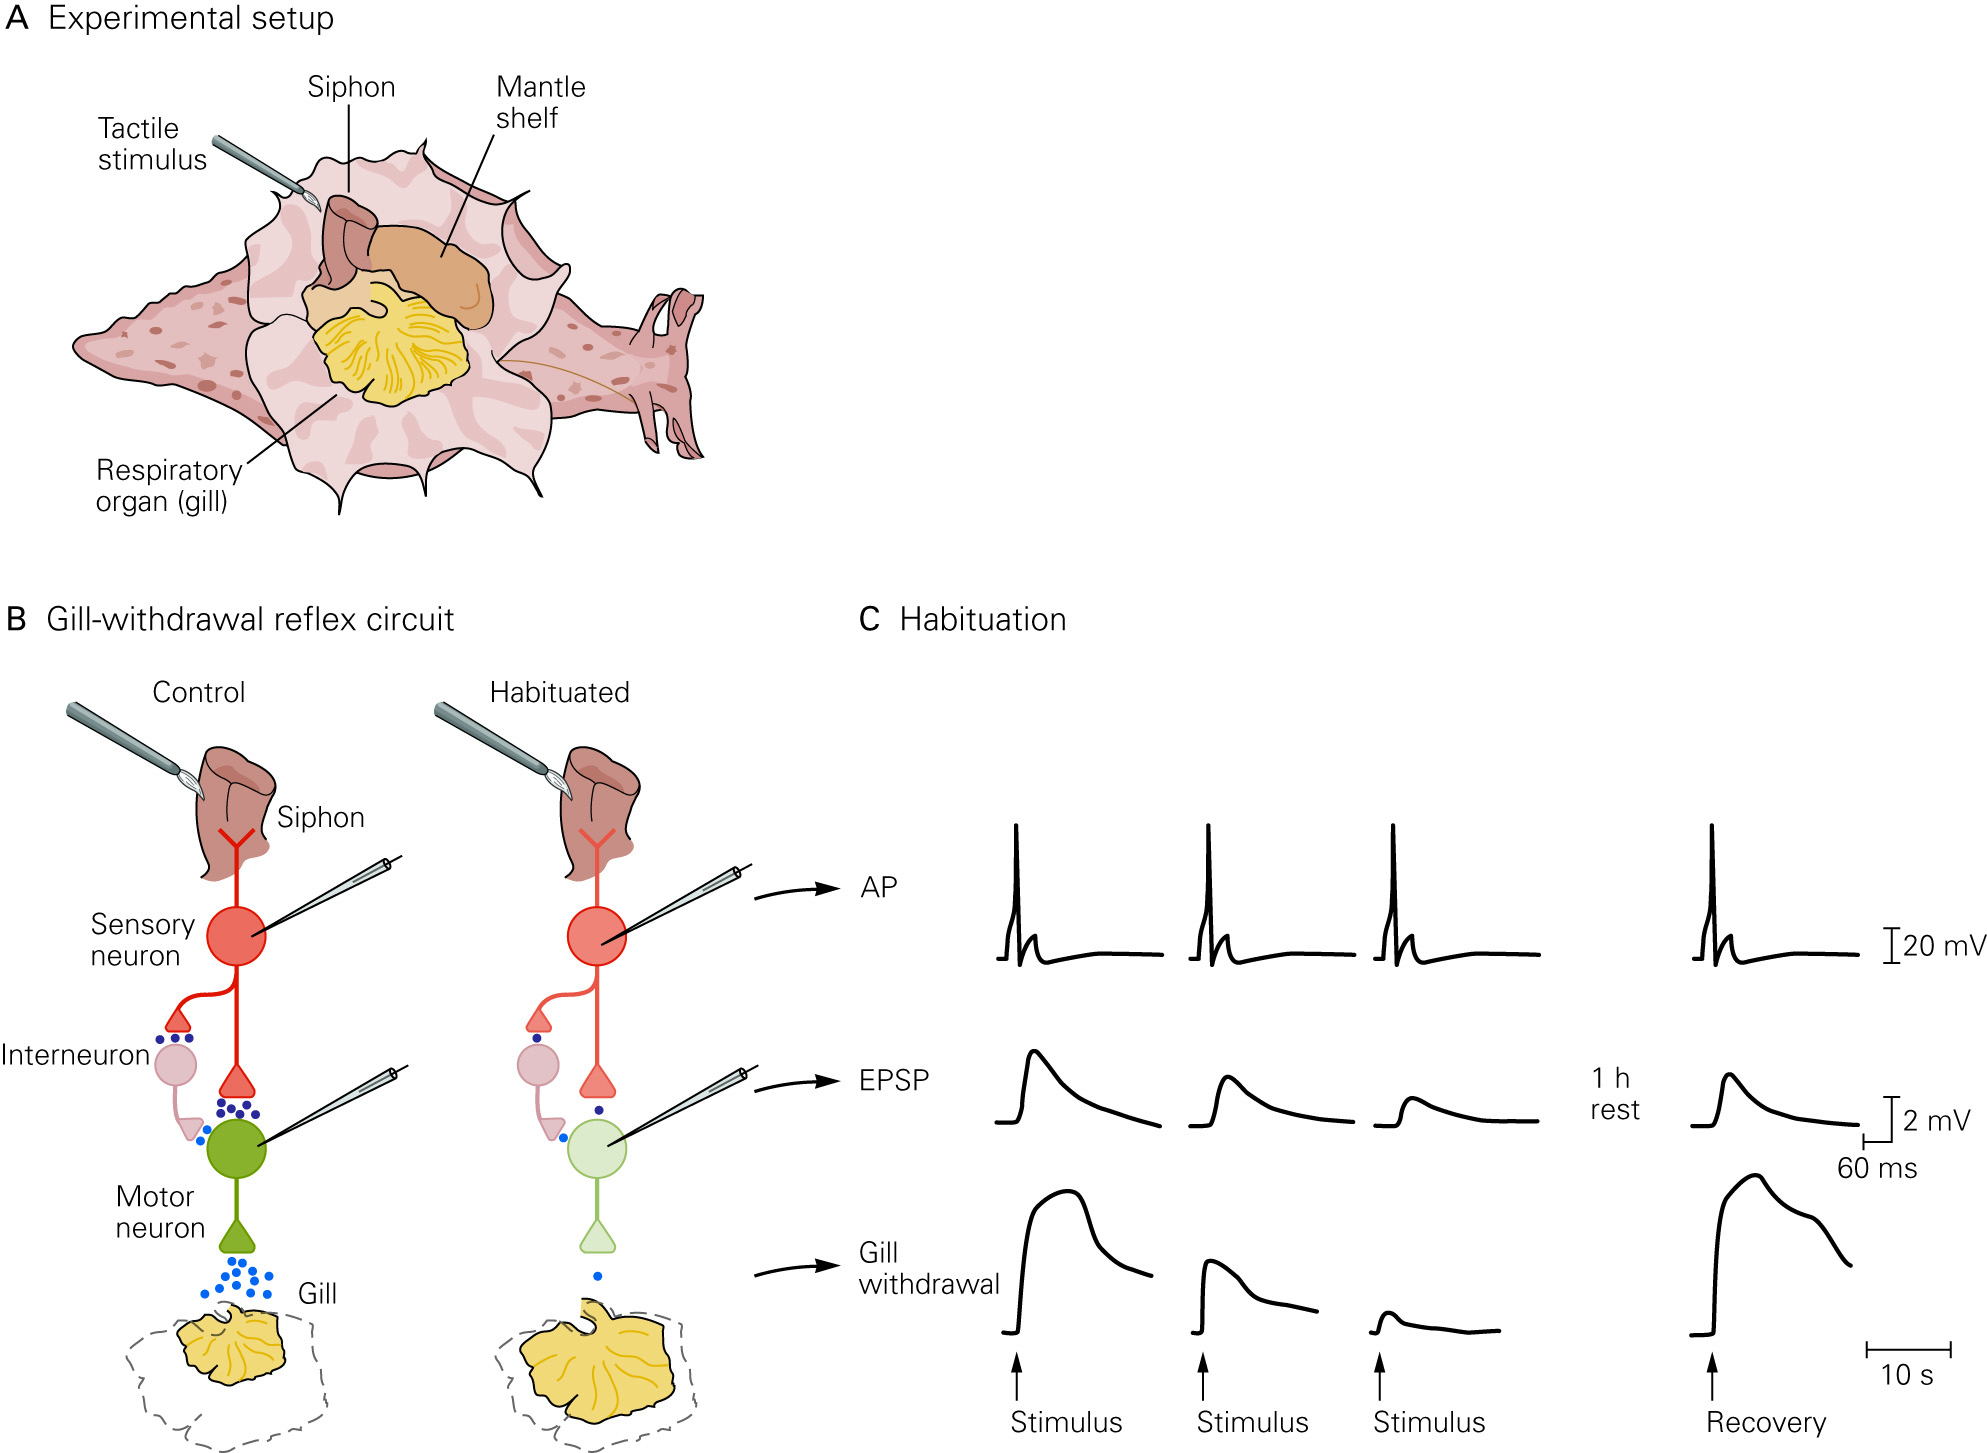
\includegraphics[scale=0.8]{Pic/6602_PNS5.jpg}
\end{figure}
\par
这种持续性的突触间功能强度的改变就是短期habituation的细胞机制。由于反射通路中会有多个点出现这种改变,所以相关的记忆也是分布的存储在整个反射通路中。多种生物实验证实了这种细胞机制也存在于其他生物中。
\par
这种突触间功能强度的改变会有多快,以及它会持续多久?在海蜗牛中连续的10个刺激会导致好几分钟的habituation。如果每10次刺激之间间隔几个小时或一天,连续刺激4次,则会造成持续时间长达3周的habituation。
\par
解剖学研究表明,长期的habituation是由于感觉和运动神经元之间的突触数量减少导致的。在没有habituation的动物中,90\%的感觉细胞会与运动细胞相连,而在经历过habituation的动物中则只有30\% 。突触数量的减少可以持续一周,有时三周之内都无法完全恢复。而敏感化则正好相反,突触数量会明显增加,这个将在后文中提到。
\par
并不是所有的突触修改的概率都是一样的。在海蜗牛中,一些突触的强度基本不随刺激的重复而变化,而另外的一些与学习相关的突触在少量的刺激下都可以长生持久而又强烈的突触强度增加。
\subsubsection{敏感化涉及到突触前膜的突触传输的增强}
当动物多次接触到有害刺激的时候,动物对这个有害刺激及其伴随刺激的反应强度都会增强,这个过程就叫做sensitization。和habituation一样,sensitization既可以是短期的,也可以是长期的。sensitization的细胞机制与habituation的细胞机制类似,只不过在数量上是正好相反的。
\par
至少三种调节性的中间神经元参与了sensitization,其中研究最透彻的神经元是以五羟色胺(serotonin)5-HT作为神经递质。5-HT能神经元在感觉神经元中分布非常的广,包括感觉细胞的突触前膜的轴轴突触。在物理刺激过后,中间神经元释放5-HT。这些5-HT会耦合到激动G蛋白受体,从而增加腺苷酰环化酶(adenylyl cyclase)的活性。腺苷酰环化酶活性增加的结果就是产生了第二信使cAMP(环磷酸腺苷),而cAMP则继续激活cAMP依赖的PKA(蛋白激酶A)。5-HT还激活第二种G蛋白偶联受体,并最终导致了磷脂的水解以及蛋白激酶c(PKC)的激活。
\par
由PKA及PKC调节的蛋白磷酸化从两个方面增强了感觉神经元的递质的释放。
\begin{enumerate}
	
	\item  PKA磷酸化钾离子通道,导致其关闭。这样增大了动作电位,并增强了钙离子通过电压门钙通道的内流。而钙离子会促进递质的释放。
	\item PKC引起的蛋白磷酸化直接增强递质的释放。
\end{enumerate}
这些由于5-HT释放所导致突触前膜的改变能够维持几分钟。重复的有害刺激下能够维持到好几天。
\begin{figure}
	\centering
	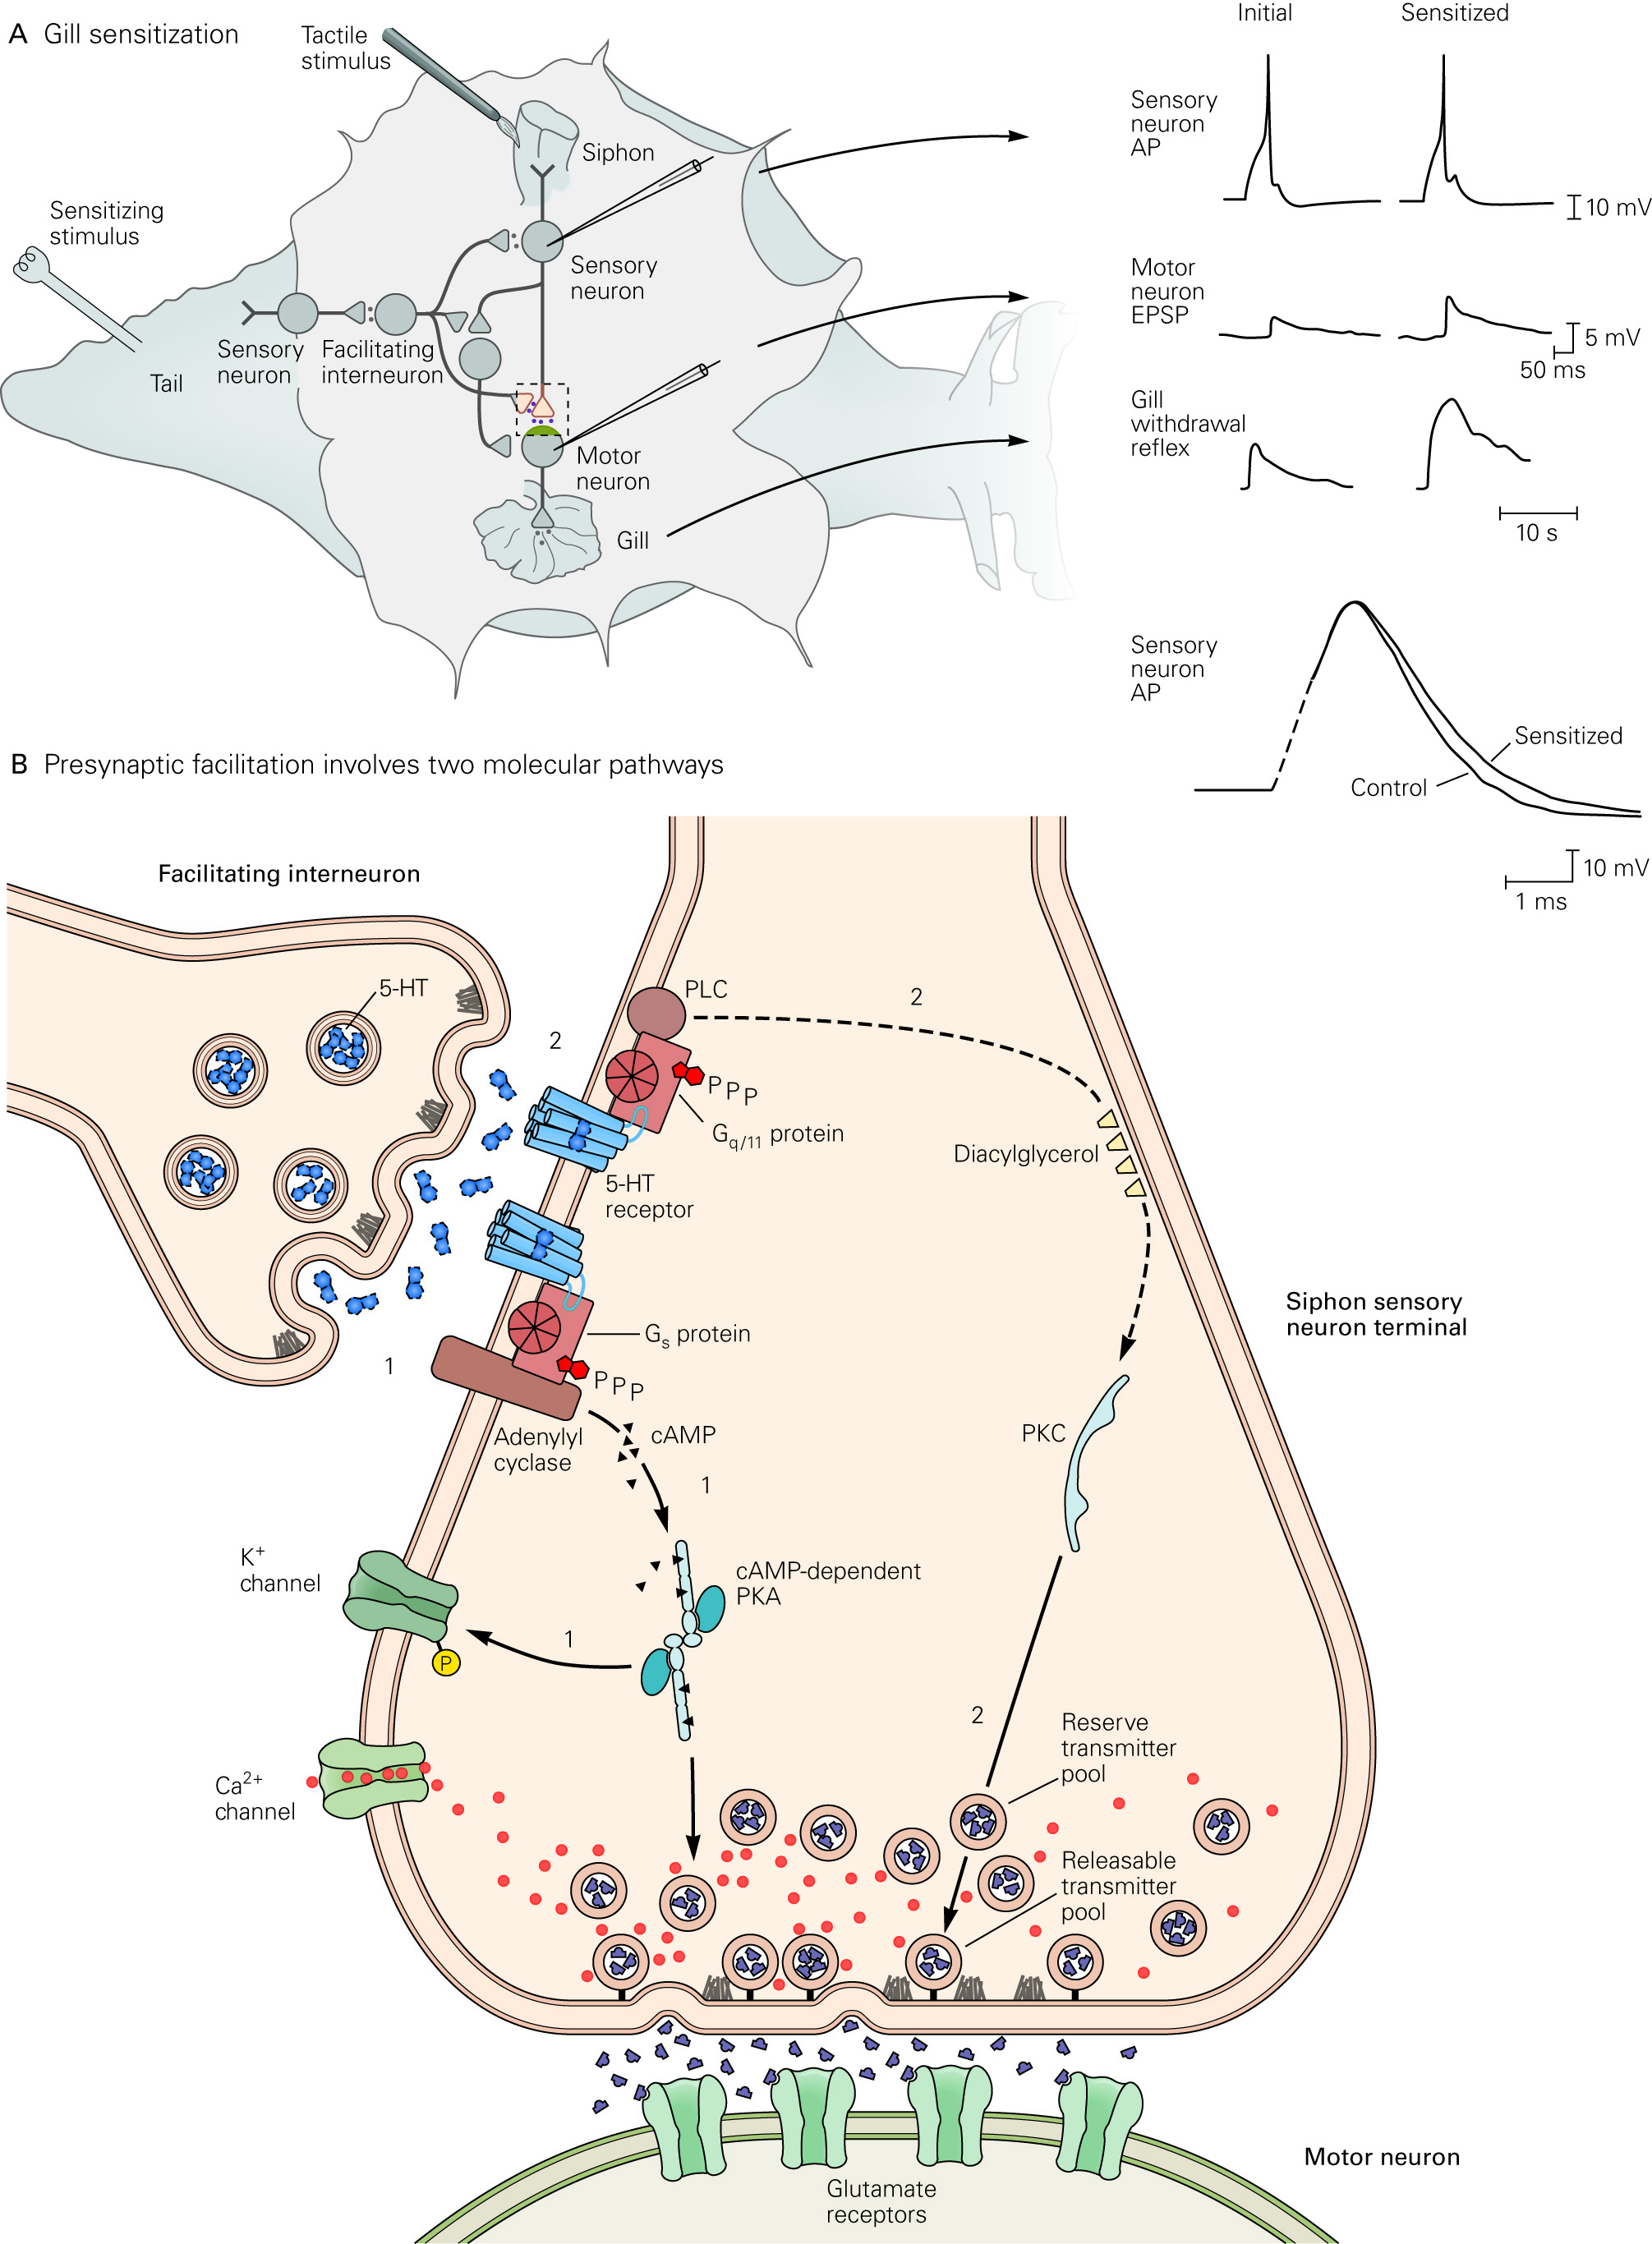
\includegraphics[scale=0.8]{Pic/6604_PNS5.jpg}
\end{figure}
\subsubsection{经典条件发射牵涉到突触前和突触后的突触递质释放的增强的协同作用}
经典的条件发射比学习更复杂,因为它牵涉到两个刺激。在海蜗牛的实验中,经过多次CS和US的协同刺激过后,单独CS刺激下所引发的活动甚至比单独US所引发的活动还强。而且实验中还发现,US和CS出现的时机也是非常重要的。为了达到有效刺激,CS必须出现在US之前的0.5s时间窗内。在此时间窗内,CS与US所引起的信号将会重合。强US刺激5-HT能中间神经元,并形成暂时的sensitization。但是,如果US是紧接着CS出现的话,中间神经元所释放的5-HT甚至能够激发更大的突触前易化作用,这个现象叫做活动相关的易化(activity-depedent facilitation)。
\begin{figure}[h]
	\centering
	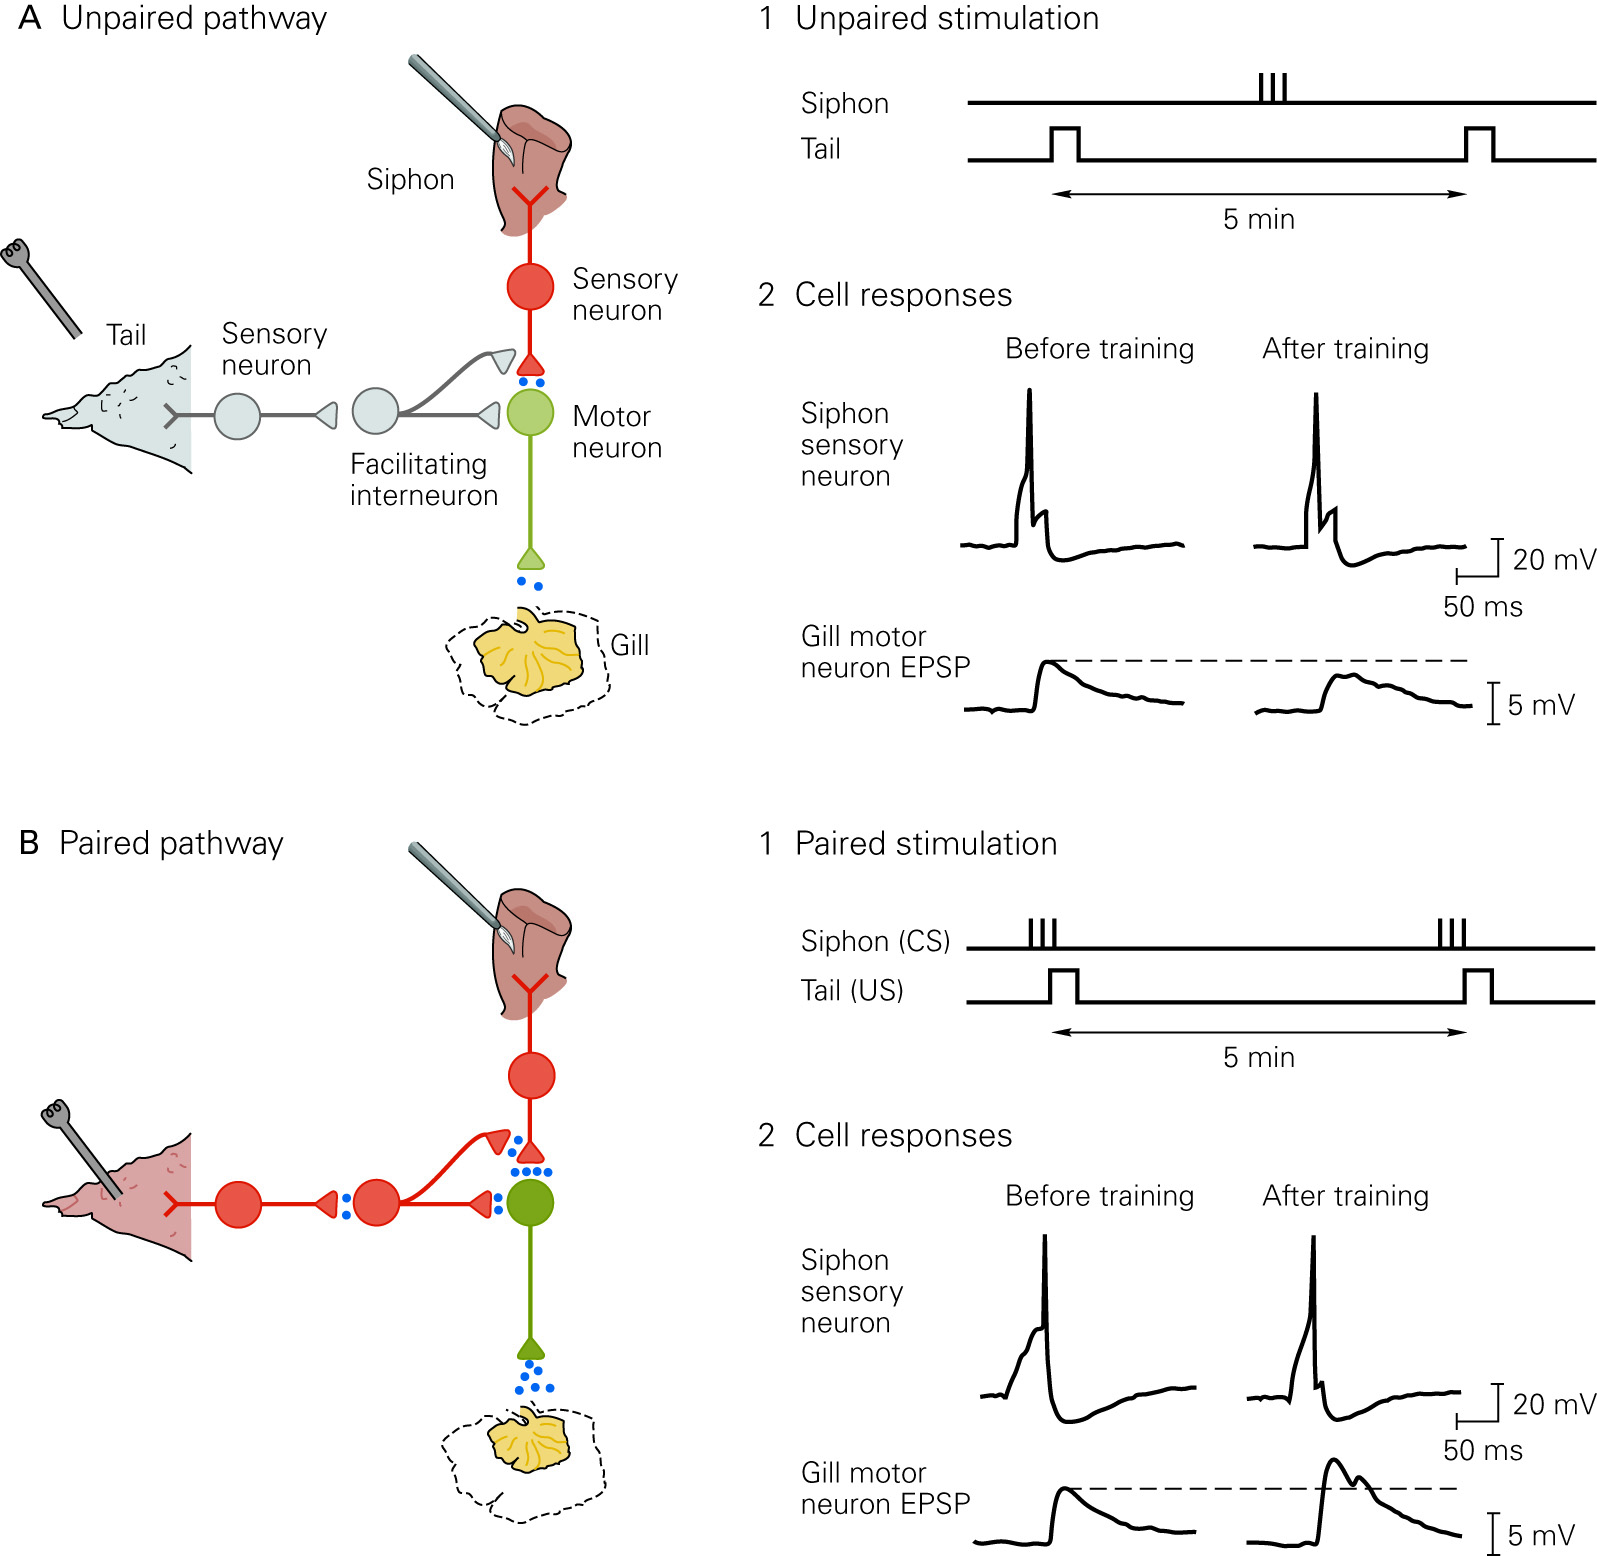
\includegraphics[scale=1]{Pic/6605_PNS5.jpg}
\end{figure}
为什么会出现这样的结果?在US刺激之后会释放5-HT,同时CS动作电位会引发感觉神经元突触前膜钙离子的内流。然后钙离子会绑定调钙素(calmodulin),然后这个复合物会绑定到腺苷环化酶。这样会促使腺苷环化酶对US刺激下生成的5-HT反应更加强烈。因此,cAMP的生成大大增强,并最终导致了突触前膜的易化。如果时间窗不重合或者时间顺序相反,则不会有这样的效果。
\par
因此,经典条件反射的sensitization在单突触通路上的细胞机制如前所述。其中腺苷环化酶起到了一个碰撞检测的作用,来检测US与CS之间是否重合。除了突触前膜的改变外,突触后膜也会做相应的改变,这里按下不表,留在67章讲LTP(long term potentiation)再去提。
\subsubsection{隐式记忆的长期存储会牵涉到染色结构和基因表达}
所有类型的学习最终都会牵涉到重复经验从短期记忆转变到长期记忆这一个过程。在海蜗牛中,这一个过程体现在长期的敏感化上。长期敏感化有着短期敏感化的所有特点,但是他还有自己的一个特殊的地方,就是长期敏感化会导致新的突触连接的生成。
\par
将短期记忆转换为长期记忆的过程,叫做固化(consolidation),这一个过程需要通路中的神经元合成mRNA和蛋白质。因此,特殊的基因表达对于长期记忆来说是必要的。这个记忆转换过程依赖于cAMP水平的长期升高,从而导致PKA的长期激活,并最终使得PKA的催化子单元进入到感觉神经的细胞核之中去。同时,它间接的激活了第二种蛋白激酶MAPK(mitogen-activated protein kinase)----丝裂原活化蛋白激酶,这个酶主要是用来调控细胞的有丝分裂。在细胞核内的PKA催化子单元会磷酸化,从而激活转录因子CREB-1(cAMP response element binding protein 1),这个转录因子会绑定到一个叫做CRE的启动子上。
\par
为了启动基因转录,磷酸化的CREB-1吸引一个转录协同激动子-CREB绑定蛋白(CBP)到启动子区域。CBP有两个对于促进基因转录激活非常重要的特性。 它吸引RNA聚合酶II到启动子区域,添加了乙酰基团到他的基质蛋白的特定赖氨酸余部,从而起到了乙酰转移酶的作用。CBP的一种最重要的基质蛋白是组蛋白,而组蛋白是核苷酸的一部分,核苷酸又是染色体的组成单元。这些组蛋白包含一系列的带正电的基础余部,这些余部与带负电的DNA磷酸根进行强烈交互作用。而这个交互作用使得DNA机密的围绕在核苷酸的周围,防止必需的转录因子接触到相应的基因位点。CBP到CREB-1的绑定造成了组蛋白的磷酸化,从而导致核糖体的一系列结构和功能的变化。乙酰化中和了组蛋白赖氨酸余部的负点,从而减少了组蛋白与DNA的亲和性。同时,特定类型的转录启动子能够绑定到乙酰化的组蛋白上,从而促进核苷酸在启动子附近的位置重排。在这些因素的影响下,基因转录的活性得到了很大的增强。
\begin{figure}
	\centering
	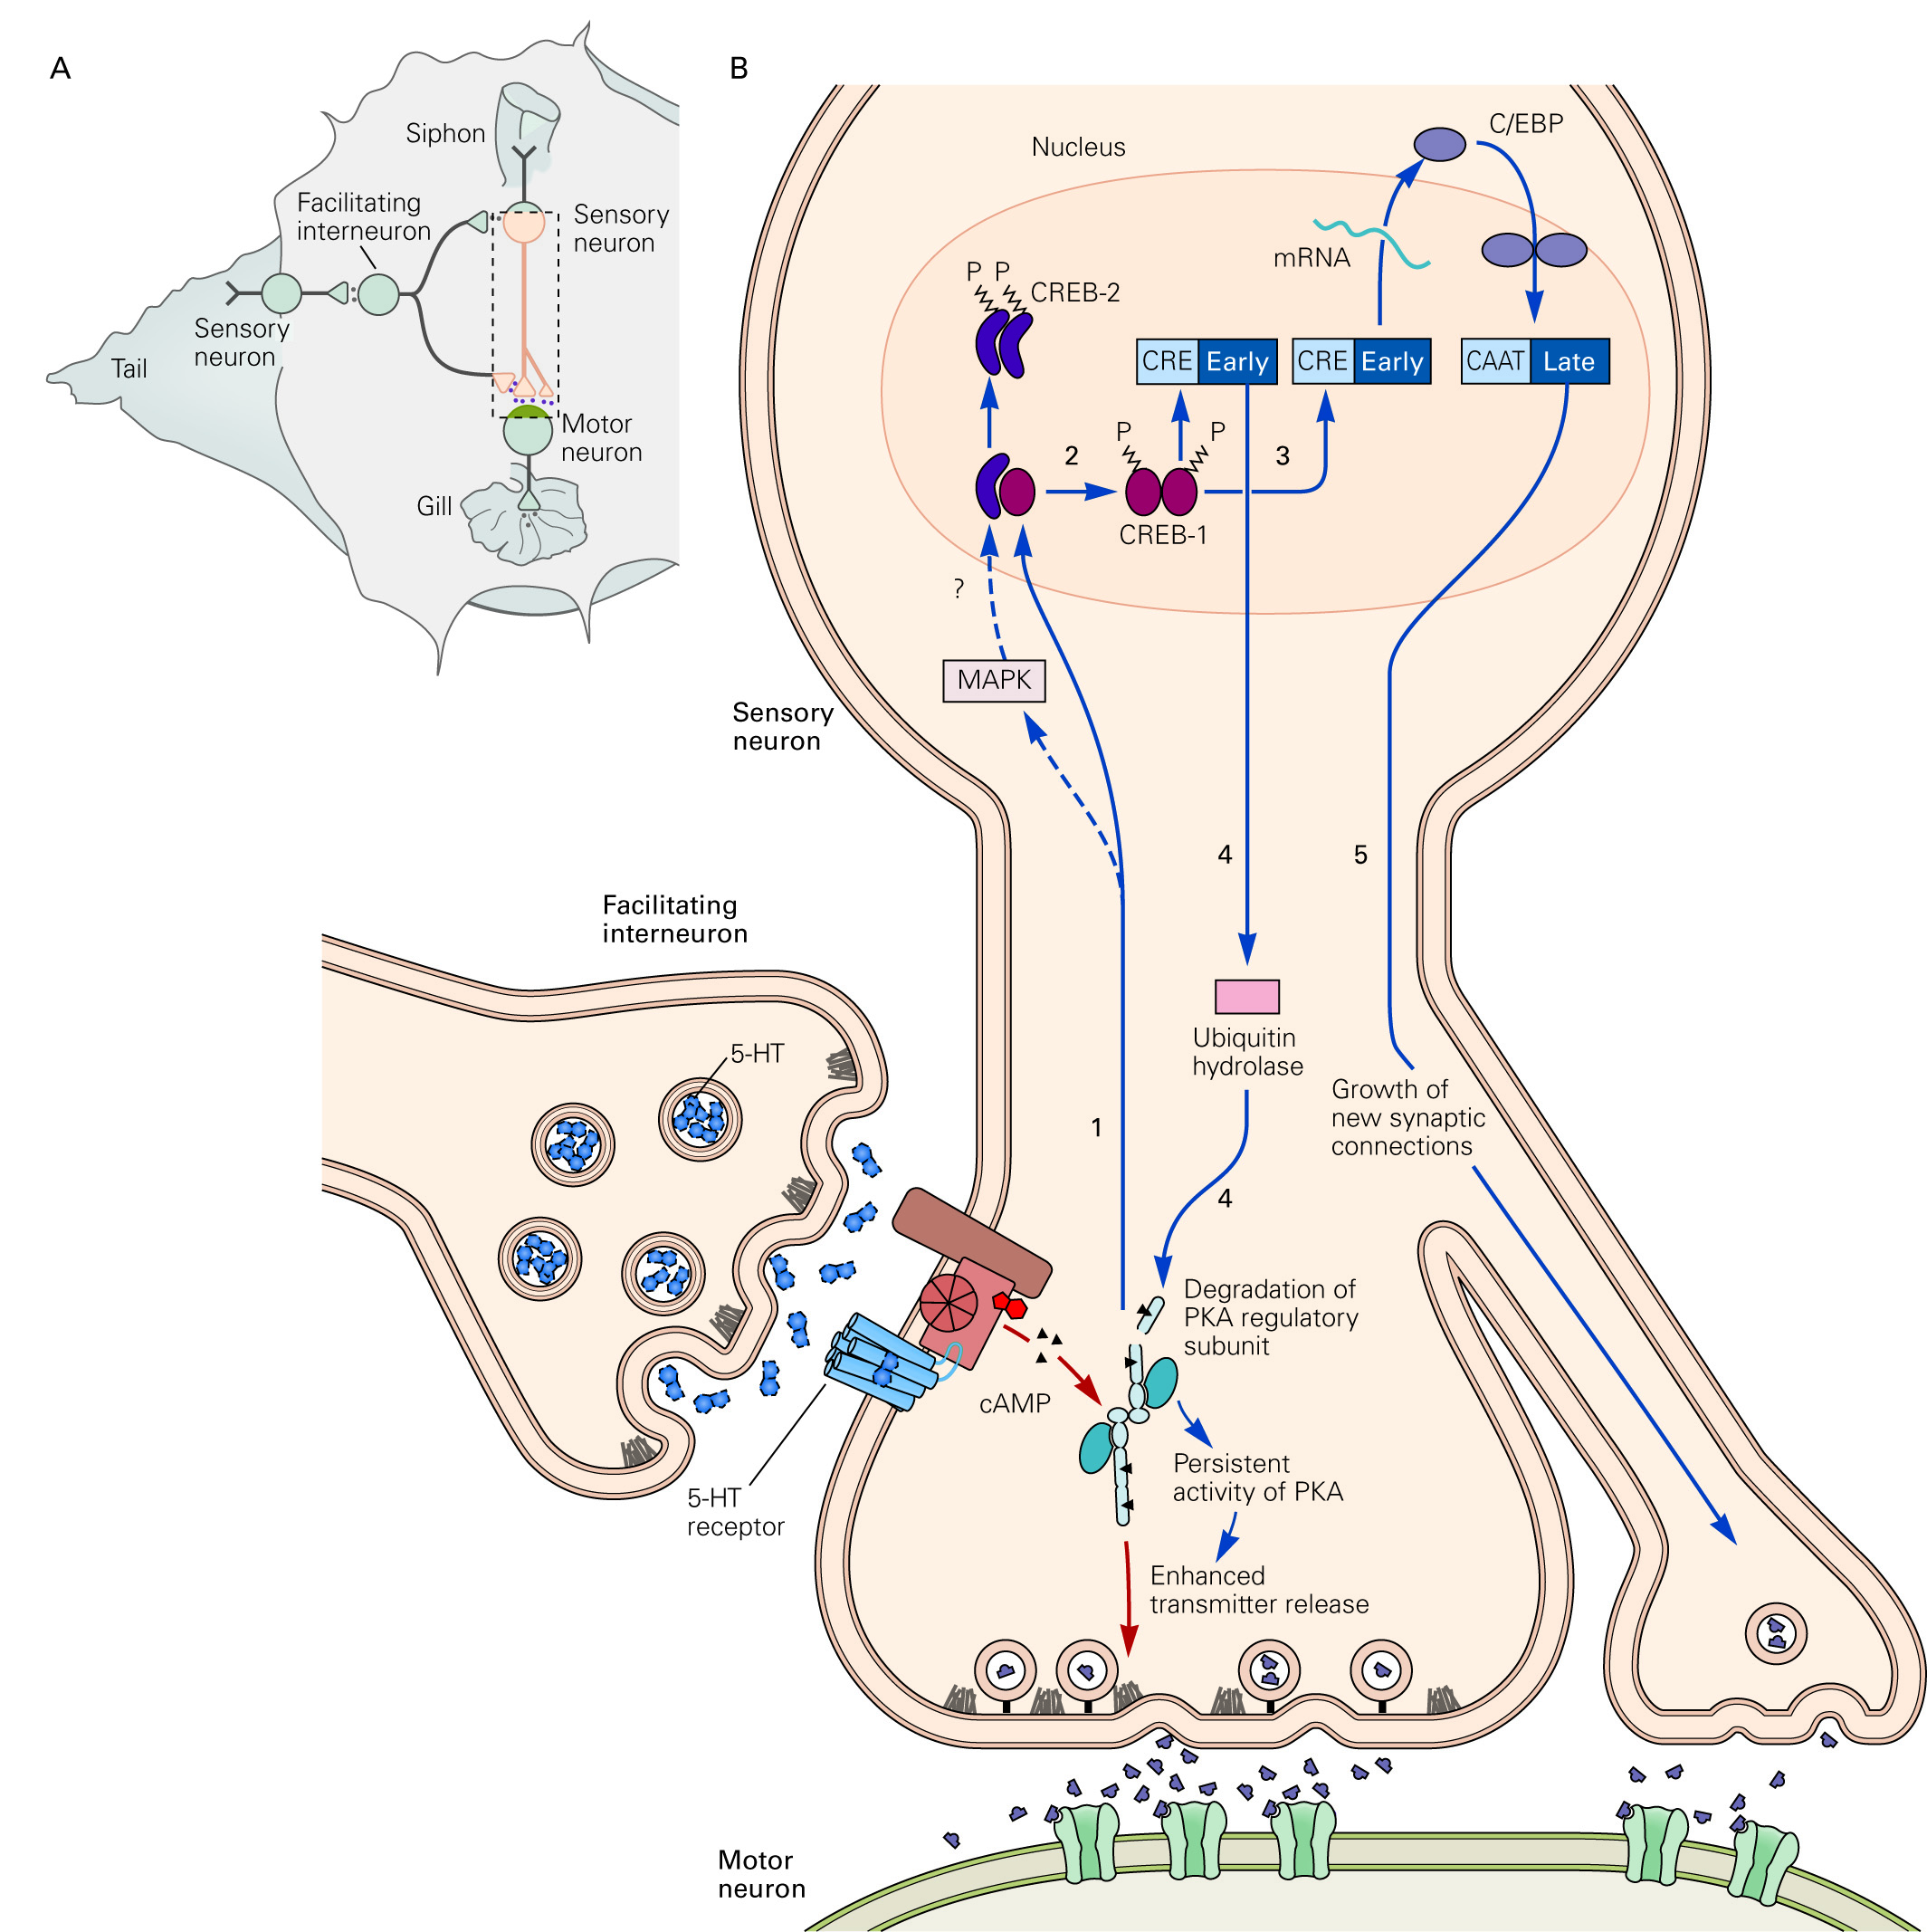
\includegraphics[scale=0.9]{Pic/6606_PNS5.jpg}
\end{figure}
\begin{figure}
	\centering
	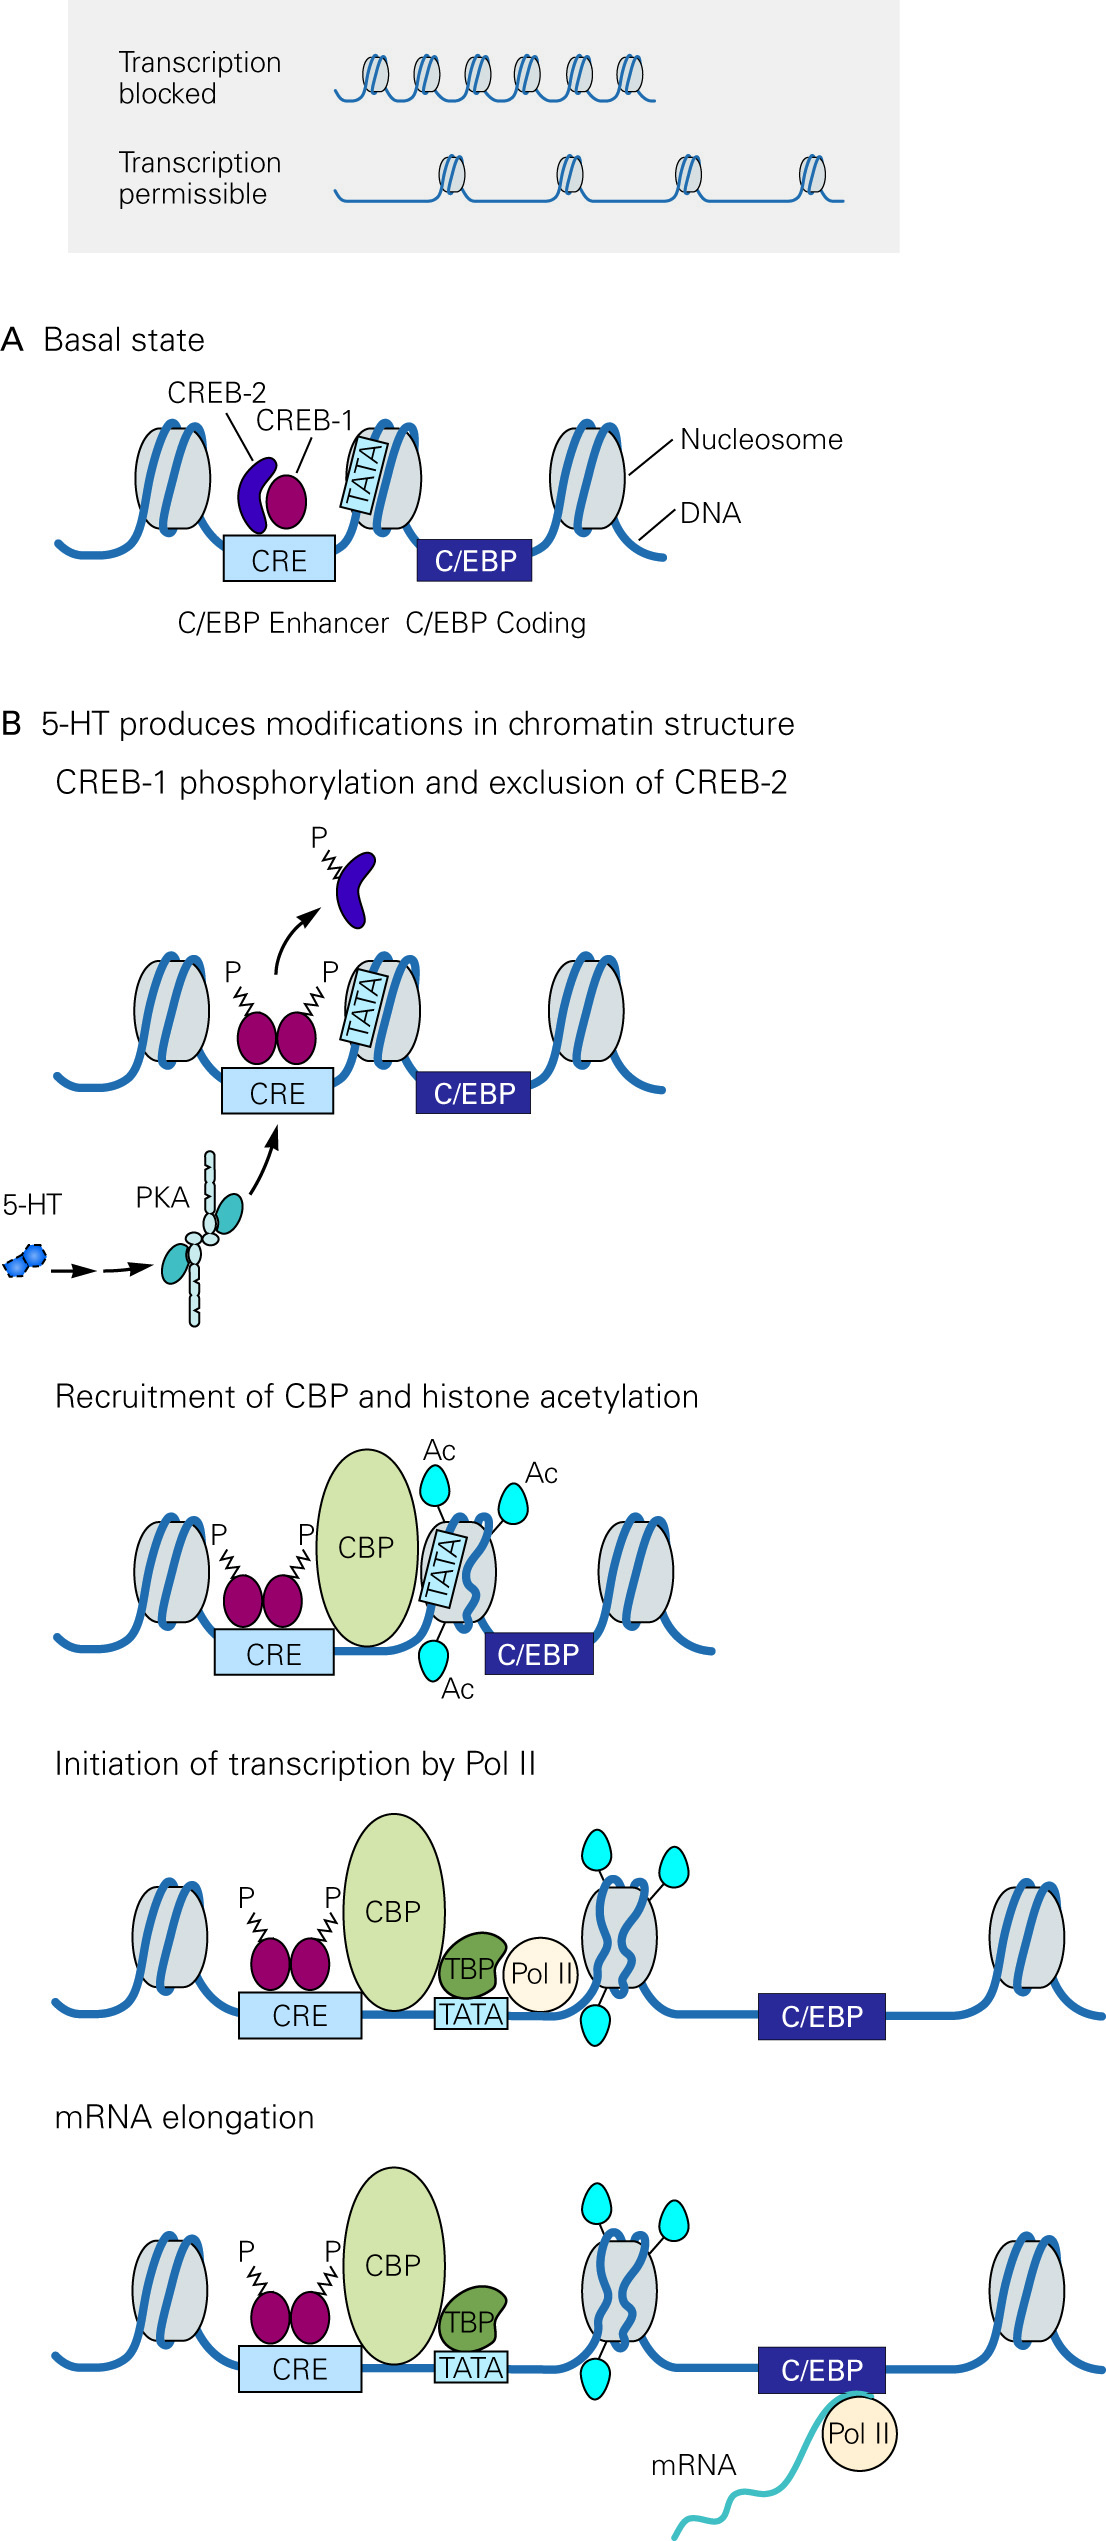
\includegraphics[scale=0.9]{Pic/6607_PNS5.jpg}
\end{figure}
\par
PKA对转录的促进依赖于它间接激活MAPK通路的能力。MAPK磷酸化转录因子CREB-2,从而减轻了CREB-2对于转录的抑制作用。综上,CREB-1的的激活以及CREB-2活动的抑制引发了学习和记忆的新的基因的表达。
\par
CREB-1和CREB-2这两个启动子和抑制子的存在表明长期记忆存储的基因表达水平是能够被调节的。这个推论符合我们日常生活的经历,即短期记忆转化为长期记忆会受到注意力、情绪和场景的影响。
\par
在CREB-1激活所引起的基因表达中,有两个基因在记忆的长期存储的初始相中起了重要作用。一个基因对应范素羧基端的水解酶,另外一个基因对应的是转录因子CAAT盒状增强绑定蛋白(C/EBP),这个C/EBP对于新突触形成所需的蛋白合成非常重要。同样见上图。
\par
范素羧基端水解酶会促进范素调控的蛋白降解,从而增强PKA的激活。PKA有四个单元:两个监管子单元抑制两个催化单元。在长期训练和水解酶的作用下,感觉神经元里将近25\%的监管子单元都会降解。因此,被释放的催化单元能够磷酸化那些对增强递质释放和增强突触强度的蛋白,特别是CREB-1,这种效应在cAMP水平回到正常水平之后尤为重要。总的来说,基本活性酶的生成是长期记忆最简单的分子机制。
\par
第二个基因所表达的转录因子C/EBP带来的效果会更持久。这个转录因子的同二聚体和和另外一个转录因子形成的异二聚体被称作\textit{activating factor}。在这些转录因子的共同作用下,下流基因的表达得到了很大的增强,并最终引发了新的突触连接的生成。
\par
在长期敏感化作用的诱导下,海蜗牛感觉神经元的突触前终端的数量得到了翻倍。同时为了适应这种数量上的变化,运动神经元的树突也增长了很多。因此长期的结构变化会在突触前和突触后都出现。而长期的习惯化的作用下,海蜗牛的突触连接的数量会下降1/3.
\subsubsection{长期突触易化是突触相关的}
在哺乳动物中,一个典型的神经元会有10000多个突触。人们很自然的提出下面的这个猜想:长期记忆的存储与具体突触有关,而不是相关神经元的所有突触。证明方法直觉上来说很简单,就是先sensitization之后,分别测试不同突触的强度。Kelsey Martin及她的同事设计了这种实验,这里就略去详细的实验设计。结果表明:长期和短期的突触易化只出现在传输通路中的相关突触上面。对于这个结果,人们不禁要问:是什么机制可以引发这种结果呢?
\par
Martin及她的同事继续相关实验,得到如下结果:新合成的基因表达附属品,例如mRNA和蛋白质,会被快速轴向传输运输到所有的突触上。但是为了利用新合成的蛋白和mRNA,突触必须要被5-HT所标记。这个现象叫做\textit{synaptic tagging}或者\textit{synaptic capture}。现在问题来了:为什么5-HT能够促进突触对基因表达产品的利用。当PKA抑制剂使用在被5-HT标记过的突触上时,该突触则无法继续利用新合成的mRNA以及蛋白质。因此,PKA调节的磷酸化过程是控制gene副产物利用的关键。1980s Oswald Steward 通过抑制突触局部蛋白合成来观察突触反应。在正常情况下,长期易化及突触增长会持续将近72小时,但是在蛋白合成抑制剂的作用下,这些只能维持24小时。该实验说明,学习诱导的突触增长需要新的局部蛋白合成。
\par
综上,在海蜗牛中,有两套不同的突触标记机制。
\begin{enumerate}
\item 第一种持续约24小时,对于突触长期的可塑性和突触增长起引导作用。这一种需要细胞核中基因的转录和翻译,以及需要局部的PKA活性,但是不需要局部的蛋白合成。
\item 第二种持续约72小时,用来稳定第一个过程所造成的突触改变。这个过程需要局部蛋白质合成的参与。
\end{enumerate}
现在问题又来了,局部蛋白合成又是谁来监管的?
\par
\subsubsection{长期易化的维持所需的局部蛋白合成是被阮病毒类物质调节的}
在5-HT刺激后突触位点的mRNA才翻译,这个现象说明mRNA初始时应该处于休眠状态,并受5-HT所引起的一系列变化来调节。Joel Richter发现在非洲爪蛙(Xenopus)的卵子中,母系的mRNA在他的3'end上有一个短尾的腺苷酸poly(A)。这些mRNA平常处于休眠状态,直到被细胞质多腺苷酸化基础绑定蛋白(CPEB)所激活。这个激活过程是通过CPEB绑定到这些mRNA上,并引导poly(A)多聚合酶。,最终导致了poly(A)的尾端的伸长。Kausik Si及其同事发现5-HT会增加海蜗牛突触局部一种新的神经元相关的CPEB的类似物的合成。CPEB的诱导是与转录无关的,但是需要一个新的蛋白合成。通过在局部阻碍CPEB能够导致突触长期易化的失败,但并不影响头24小时的易化。
\par
CPEB是如何促使突触的长期易化的?绝大部分生物分子都只有比较短的半衰期,一般是几个小时到几天不等。而记忆却可以持续多年,如何长期的维持分子浓度?当前的绝大部分假说都依赖于一种自维持的机制来解释长期的易化现象。
\par
Si和他的同事发现海蜗牛CPEB的神经类似物拥有类似于阮病毒的自维持机制。阮病毒有两种存在形式:溶解态和聚合态,其中聚集态有自我催化功能。海蜗牛的CPEB也有两种形态:一种溶解态(无活性),一种聚合态(有活性)。这两种形态之间的切换牵涉到CPEB富含谷氨酸的N端,类似的位点也存在于其他的阮病毒蛋白之中。
\par
在未激活的突触中,CPEB是维持在溶解态的,活性程度很低。在5-HT刺激之后,CPEB的合成增加。当增加到一定浓度之后,CPEB开始聚合。聚合态的CPEB不仅能够激活休眠状态的mRNA,而且还能催化CPEB的聚合过程。正因为CPEB的这种自催化作用,突触易化才能维持一个很长的时间。这种机制不仅仅在海蜗牛上有,在其他动物上也有。
\subsubsection{哺乳动物恐惧的记忆学习需要杏仁核}
在Joseph LeDoux,Michael Davis以及Michael Fanselow等人的前期工作的基础上,我们对于哺乳动物先天恐惧和后天恐惧的传输通路有了很好的了解。其中最重要的是,这两种恐惧都涉及到杏仁核。杏仁核会参与到多种潜在有害刺激的侦测和评估。杏仁核不仅能够直接接收无意识的恐惧反应信息(如表情),还能够通过扣带回皮层间接的接受有意识地恐惧信息(如感觉)。
\par
出了天生的恐惧应答之外,杏仁核作用下的防御系统也能够快速学习新的危险。单次条件刺激就可以形成一生中的记忆。在此条件刺激下的信号既可以直接快速从丘脑传输到杏仁核,也可以间接慢速的从丘脑传输到大脑皮层然后再传输到杏仁核。
\begin{figure}
	\centering
	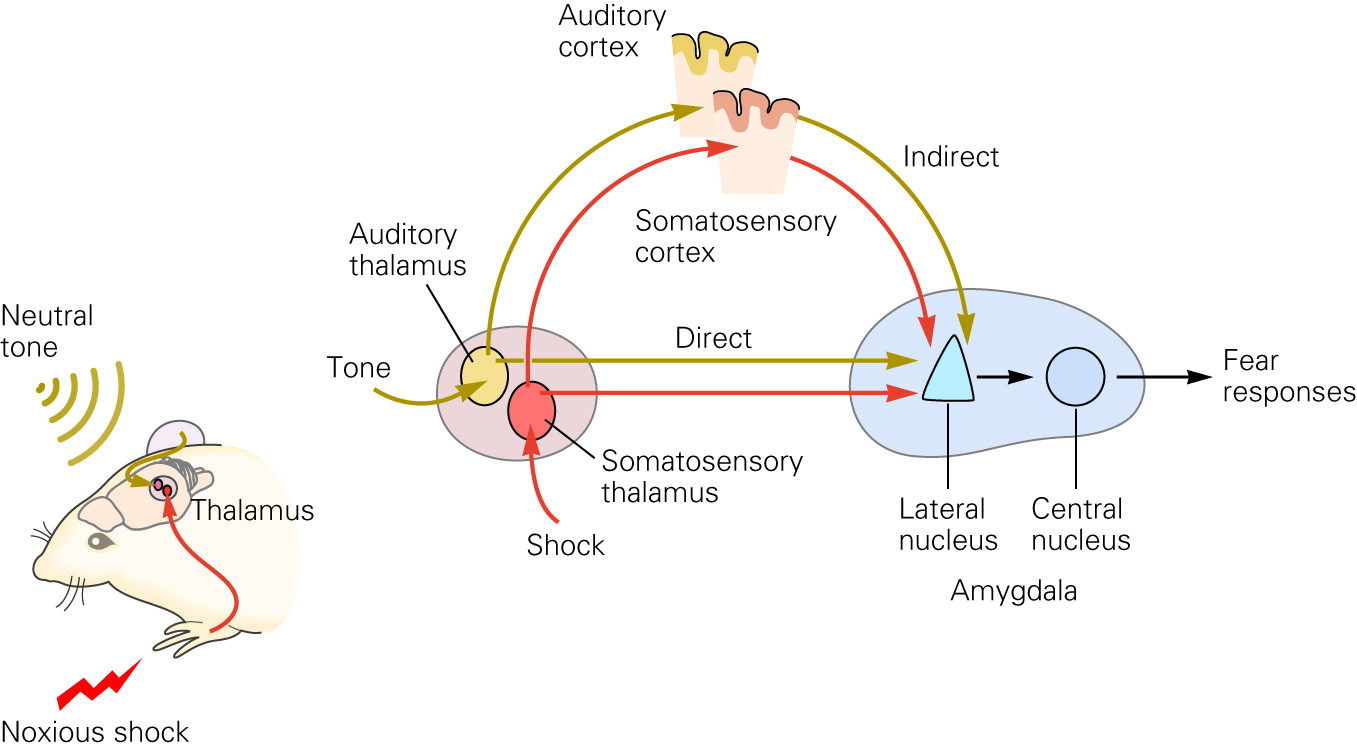
\includegraphics[scale=0.9]{Pic/6612_PNS5.jpg}
\end{figure}
学习恐惧的长期记忆也需要CREB,杏仁核中不同神经元参与长期记忆的程度与该神经元中CREB的表达水平有关,越多越好。现在问题来了,恐惧学习中突触强度的增加原因是什么?
\par
通过在杏仁核及相关通路的离体实验,学者发现在恐惧学习中突触会形成长期的突触应答强度增加,也叫做long-term potentiation(LTP)。这个概念会在67章介绍显示记忆与海马的时候详细说明。在杏仁核的外侧核团的LTP是由于突触后膜的钙离子内流引发的,这个内流是在NMDA型谷氨酸受体和L-type电压门钙通道调控的。钙离子的内流已发了一系列的生物化学反应。这些反应通过在突触后膜增加额外的AMPA型谷氨酸受体及增加突触前端的递质释放来达到增强突触传输的目的。长期的恐惧记忆以及突触变化也需要cAMP依赖的蛋白激酶和MAPK,这些物质在海蜗牛中也是必须的。
\par
我们通过实验所观察到的这些现象是记忆所需的变化,还是记忆变化所附加的现象?两个基因实验证明了LTP是恐惧学习所必需的。一个实验通过敲除NMDA受体的GluN2B子单元基因,发现会影响到恐惧调节和传输通路商的LTP的产生。而且这个基因突变只会影响到后天学习到的恐惧,而不影响先天学习到的恐惧,也不影响平常的突触传输。反过来,GluN2B的过度表达会增强恐惧学习。
\par
更让人信服的证据是经过恐惧学习的动物的离体杏仁核的LTP比没有经过恐惧学习的动物的离体杏仁核的LTP小。因为突触电位有一个上界,所以非条件刺激所产生的电位会减弱而条件刺激的电位会增强。
\begin{figure}[h]
	\centering
	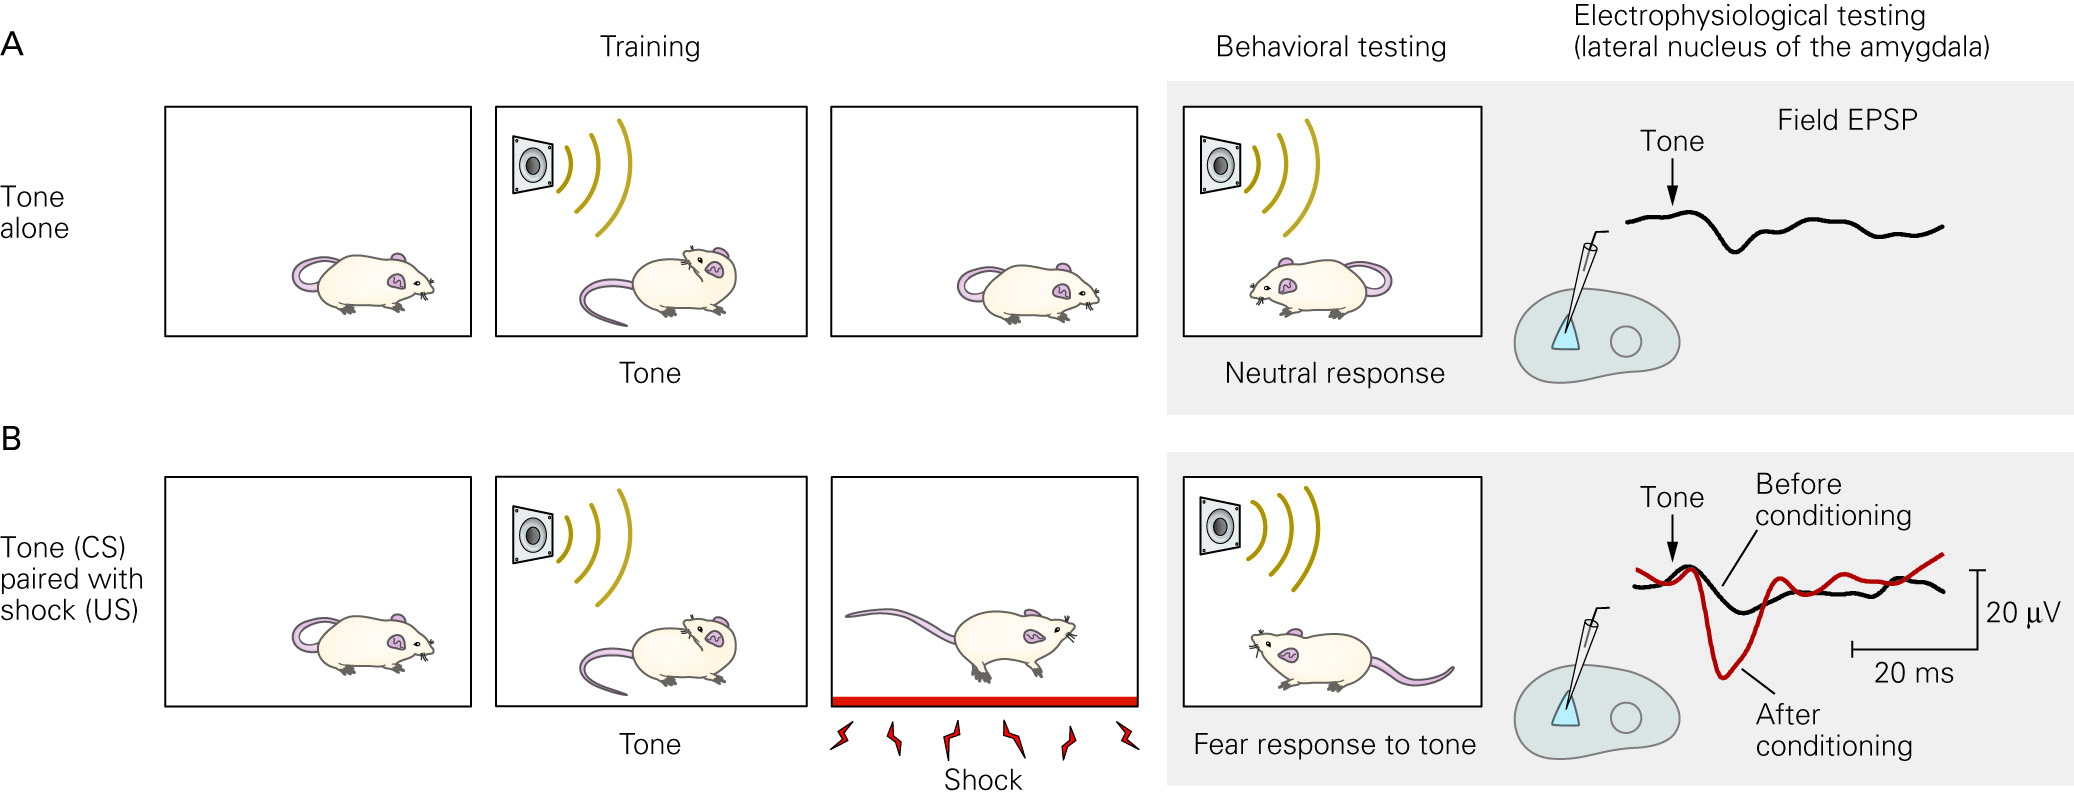
\includegraphics[scale=0.9]{Pic/6613_PNS5.jpg}
\end{figure}
\subsubsection{习惯学习和记忆需要纹状体}
这里都是一些实验,这个实验比较有趣。一个是完全凭记忆来走迷宫,一个是完全凭刺激反射来走迷宫。通过这个实验说明了纹状体在隐式记忆中起作用,而海马则在显式记忆中起作用。
\newline
\begin{figure}[h]
	\centering
	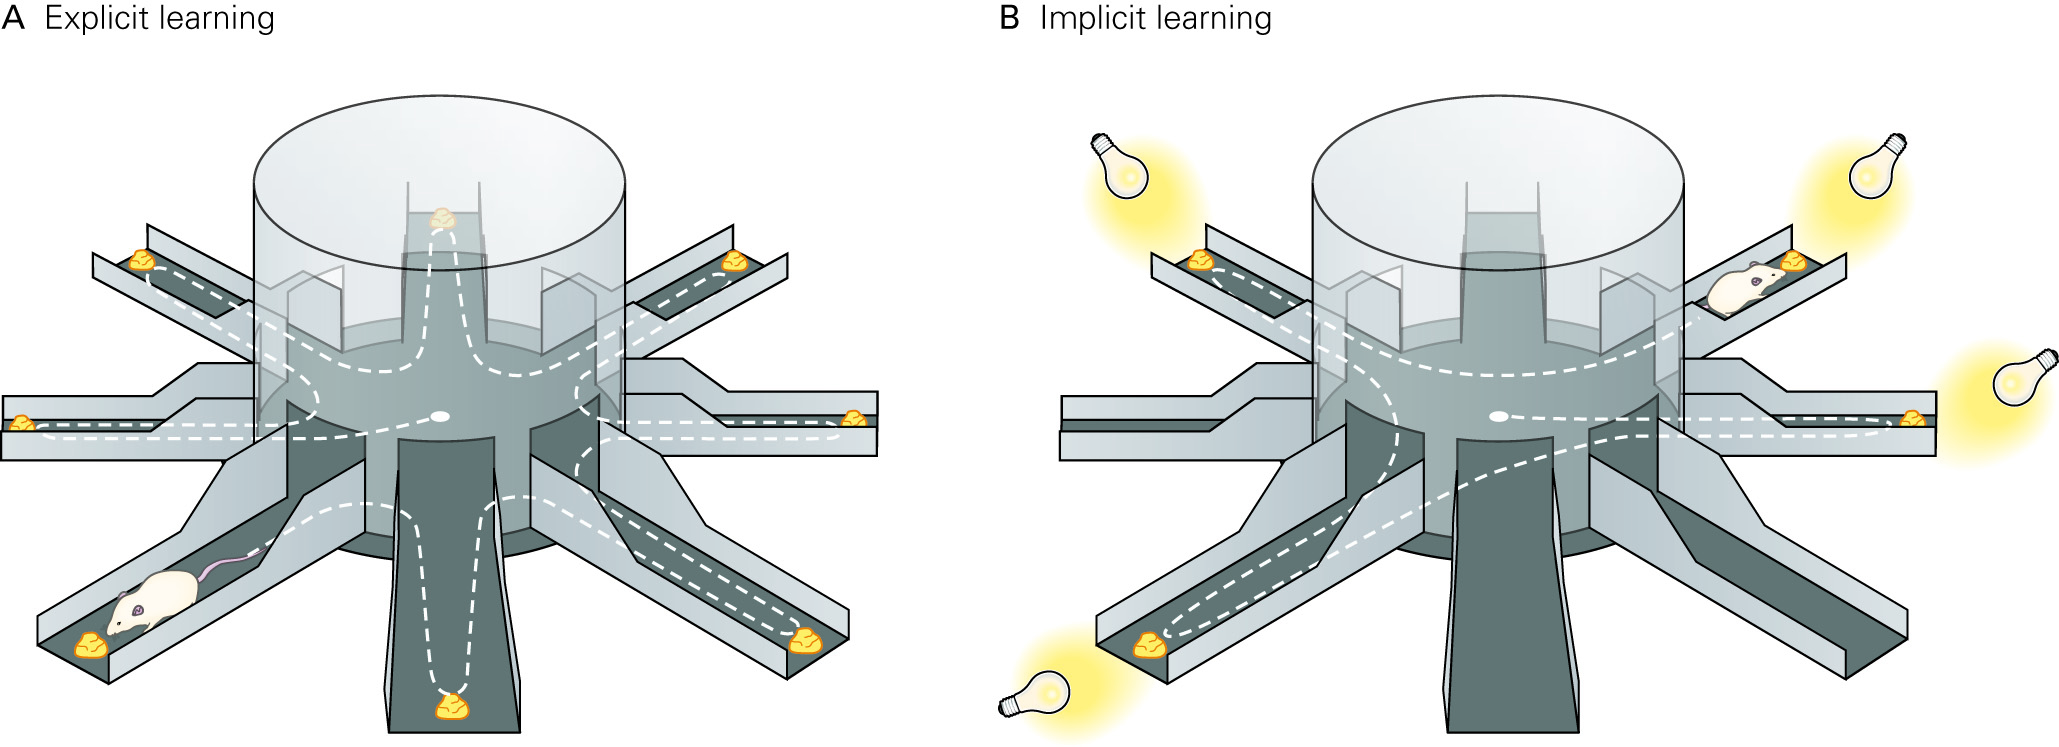
\includegraphics[scale=0.9]{Pic/6615_PNS5.jpg}
\end{figure}

\subsubsection{学习引发的大脑结构变化是个体独立性的基础}
发现经常使用某个部位会导致这个部位的脑区增大,同样如果经常不使用某个部位则会导致相应脑区缩小。而且如果多个部位被绑定来同时使用时,这几个部位之间的界限就会被抹平(这里的例子就是将两个手指绑起来)。
\subsection{前额皮层,海马以及显式记忆存储的生物学}
哺乳动物大脑中有两个结构对于记忆的编码和存储非常重要,分别是前额皮层和海马。前额皮层负责工作记忆(working memory),这些记忆维持时间非常的短,只有几秒到几分钟。而海马则负责记忆的长期存储。
工作记忆依赖于前额皮层的长期活动性增强
前额皮层的活动性增强依赖于两个机制:神经元细胞膜的内在性质以及突触之间的往返连接。
\subsubsection{神经元细胞膜的内在性质能够生成持续的电位活动}
在一些大脑皮层神经元中,一个简单的电刺激能够引起持续数秒乃至数分钟的电冲动。更奇异的是,这种持续的电冲动不会被快速激动阻滞剂及突触传输抑制剂所影响,说明这个持续性的电位活动是依赖于这个神经元的细胞膜的性质。
\par
这种现象在内嗅皮层及其明显。一般来说一个简短的去极化电流能够引起一个快速简短的动作电位。但是如果内嗅皮层的神经元暴露在乙酰胆碱的作用下时,G蛋白偶联毒蕈碱受体会被激活,并导致长达数十秒的动作电位。
\par
这种长期的动作电位依赖于一种被称为非选择性钙离子激动(ca\textsuperscript{2+}-activiated nonselective,简称CAN)的阳离子通道。这个通道的打开依赖于两个事件同时发生:一个是毒蕈碱受体必须被细胞外的乙酰胆碱激活且引发信号传递,另外一个是细胞内部的钙离子浓度增加(一般是由于初始电刺激引起的电压门钙离子通道的打开)。当这两个条件都具备的时候,钙离子通过绑定在CAN的细胞内表面来激活CAN。由于初始电刺激之后细胞内的钙离子浓度会维持一段时间,所以CAN通道所引起的阳离子内流会导致长期的去极化。如果初始刺激周期很密集的话,更多的CAN通道会被钙离子激活,从而引起次一级的动作电位。又由于动作电位会引起更多的钙离子内流,从而导致更多的CAN的开放。这是一个正反馈的过程,总的结果就是该神经元的长期firing。最近的研究表明,这种持续firing的机制也在前额皮层中出现。
\subsubsection{特殊的网络连接能够维持激活}
第二种位置长期firing的机制是神经通路之间的往返连接。这种连接结构下,神经元之间会互相刺激,类似于正反馈的效果。这种连接既可以是大区域的往返连接,也可以是局部的往返连接,详细的可以看下图。
\begin{figure}[h]
	\centering
	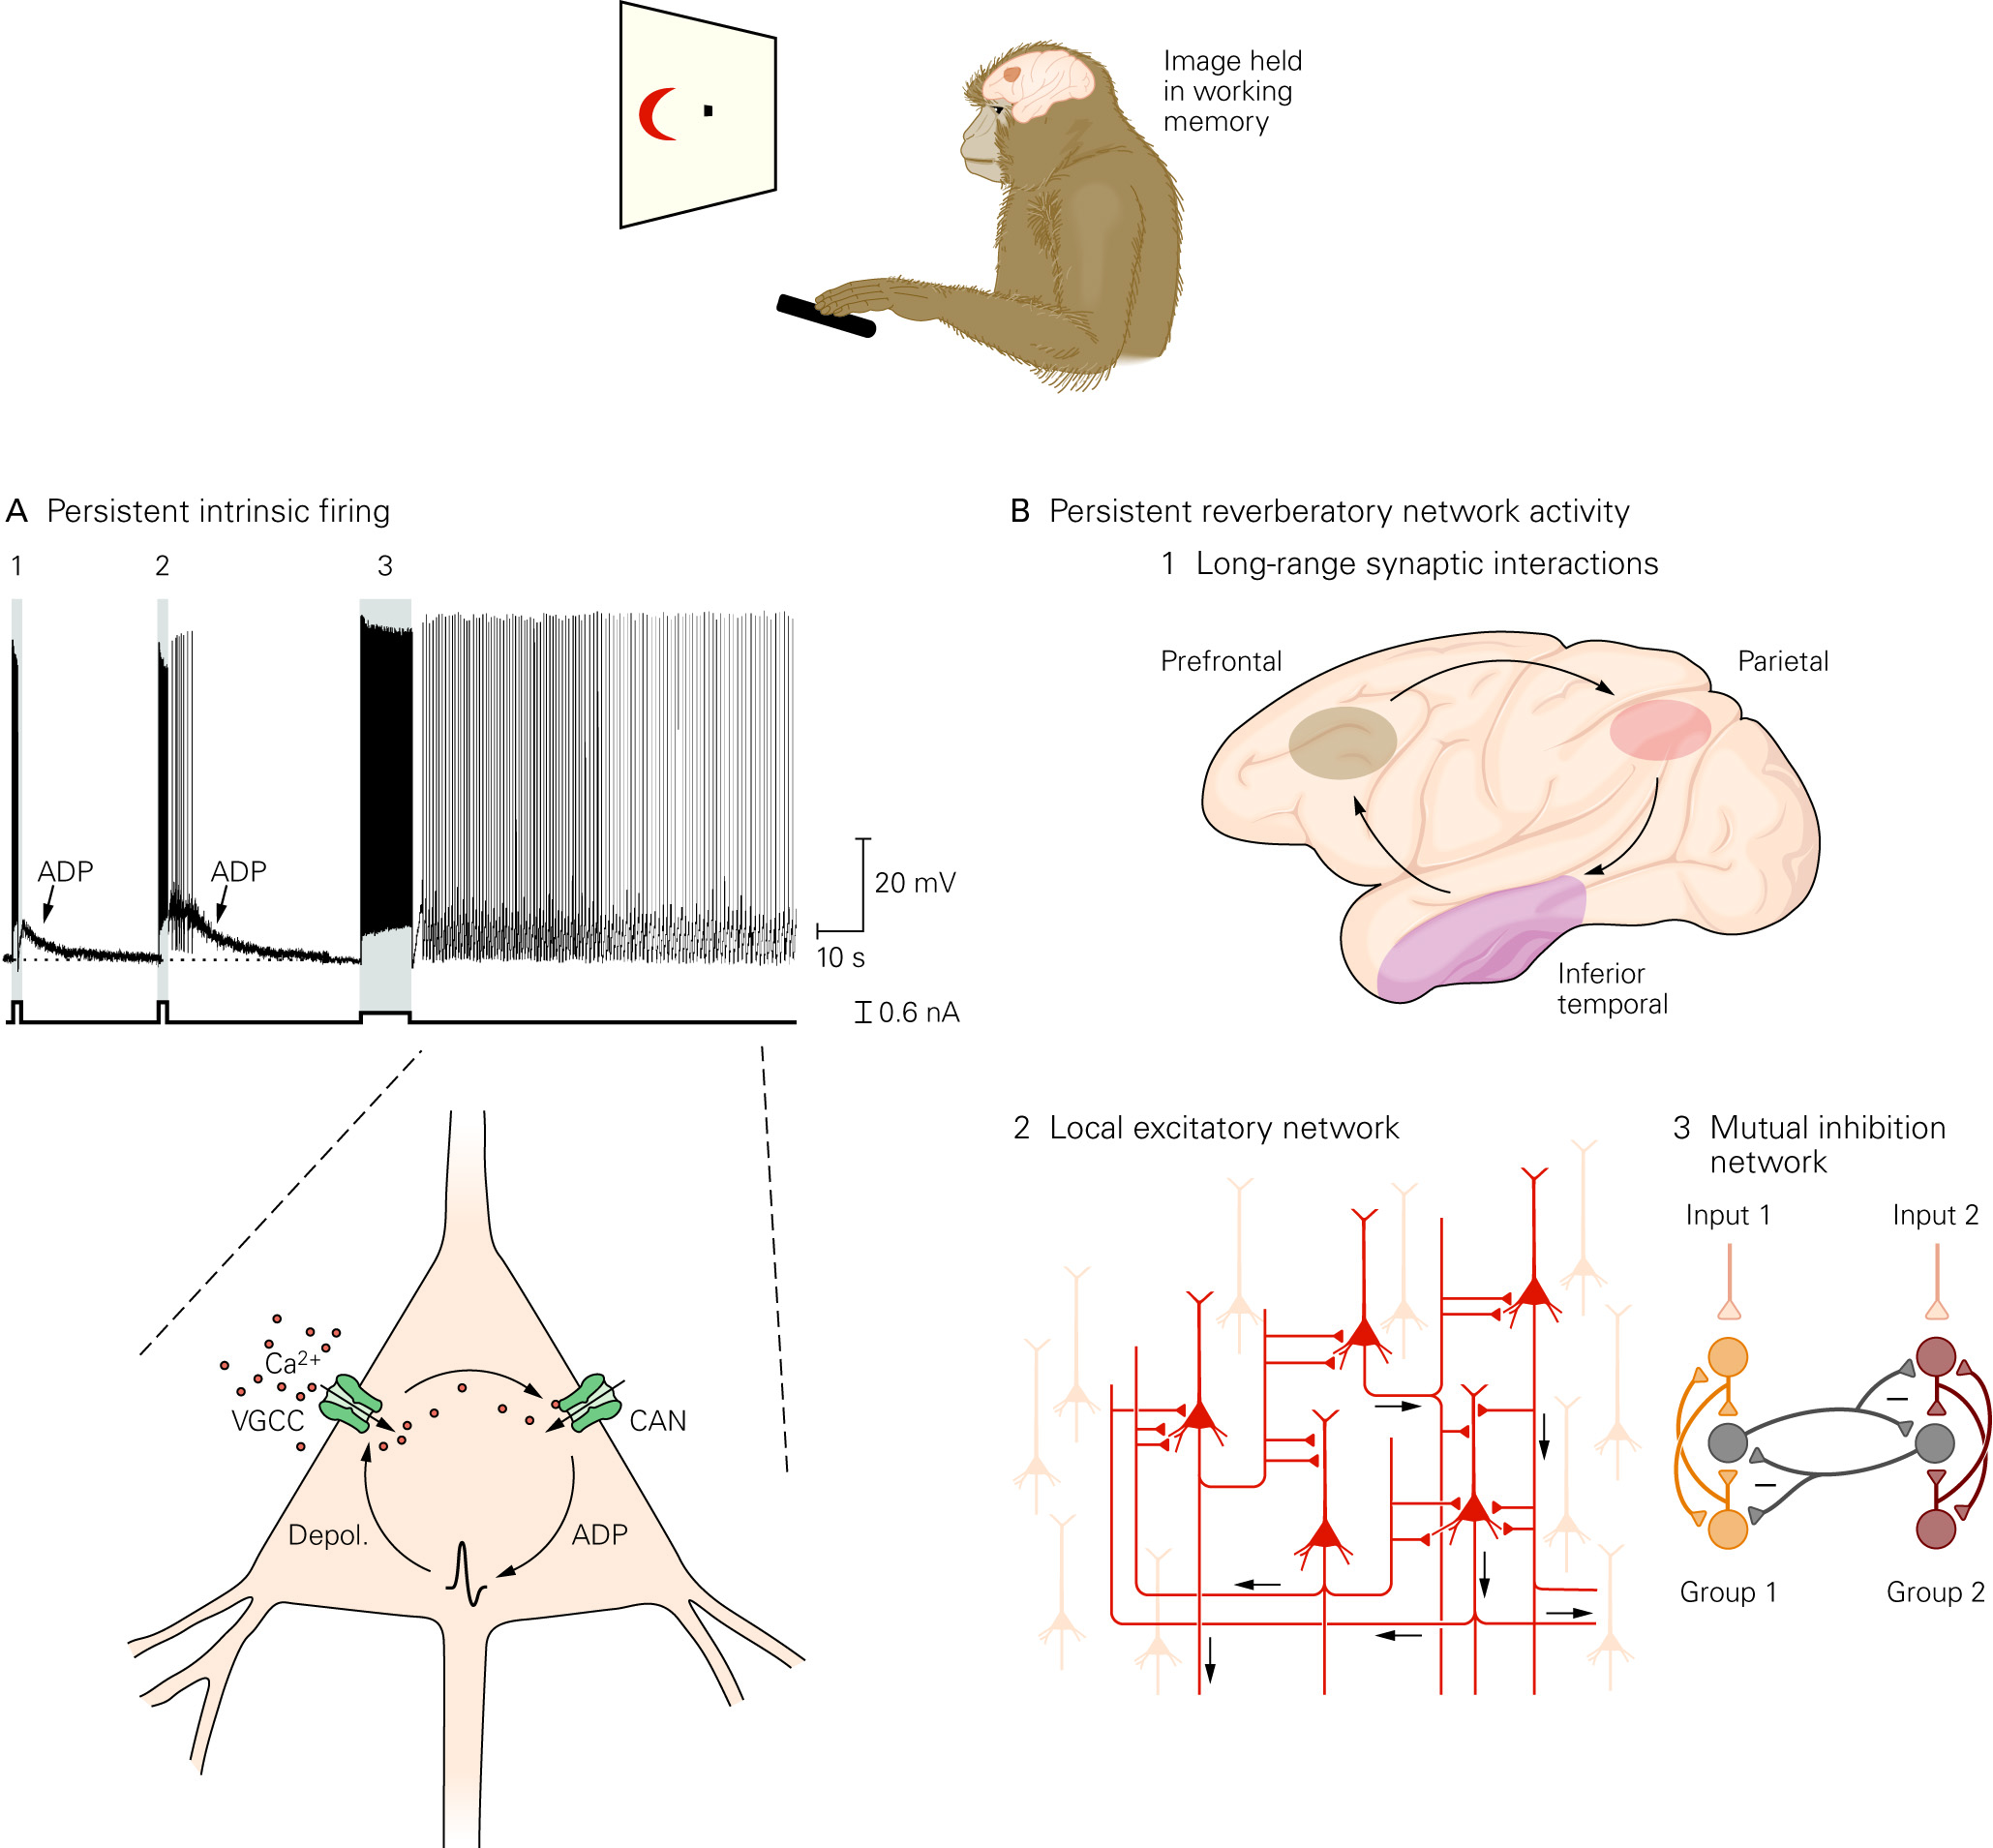
\includegraphics[scale=0.9]{Pic/6701_PNS5.jpg}
\end{figure}
还有另外的一种能够维持长期激动的往返连接的结构,这种结构中只有两类神经元。这两类神经元互相抑制,也就是keep in check。但是当其中一种神经元受到刺激时,会导致这种神经元对另外的那种神经元抑制增加,也就是负负得正的效果,这种机制叫做disinhibition。
\subsubsection{工作记忆依赖于调节递质多巴胺}
尽管神经膜内在活动与网络往返连接在工作记忆的相对重要性还不清楚,但是目前有很明显的证据表明在前额皮层的神经元的工作记忆及长期活动性依赖于D\textsubscript{1}类型的多巴胺受体。这些受体是与G蛋白和cAMP偶联的。Patricia Goldman-Rakic及其同事发现D\textsubscript{1}类型的多巴胺受体与工作记忆之间的关系呈倒U型。即只有D\textsubscript{1}类型的多巴胺受体激活数量适中时工作记忆的效率才是最高。
\subsubsection{哺乳动物的显式记忆依赖于海马不同形式的LTP}
不像工作记忆,海马区存储的长期记忆并不依赖于长期的firing,而是依赖于长期的突触连接之间强度增加。海马从临近的内嗅皮层接收多种的感觉和空间信息。海马主要的输出位点是在CA1区域的椎体细胞,而输出目标又回到了内嗅皮层,此外还有海马支脚(subiculum)。CA1区域对于学习和记忆是非常重要的,在CA1区受损的病人之中会有显著的记忆损伤,动物实验也提供了同样的结论。从内嗅皮层传递到CA1区域的信息通路有两条:一条是直接通路,另外一条是间接通路。这两条通路被并称为perforant pathways。
\par
直接通路起点在于内嗅皮层的layer III,这些起点神经元与CA1神经元的轴突末端形成突触。间接通路的起点在于内嗅皮层的layer II,并通过trisynaptic pathway最终到达CA1。整个通路的结构见下图。
\begin{figure}[h]
	\centering
	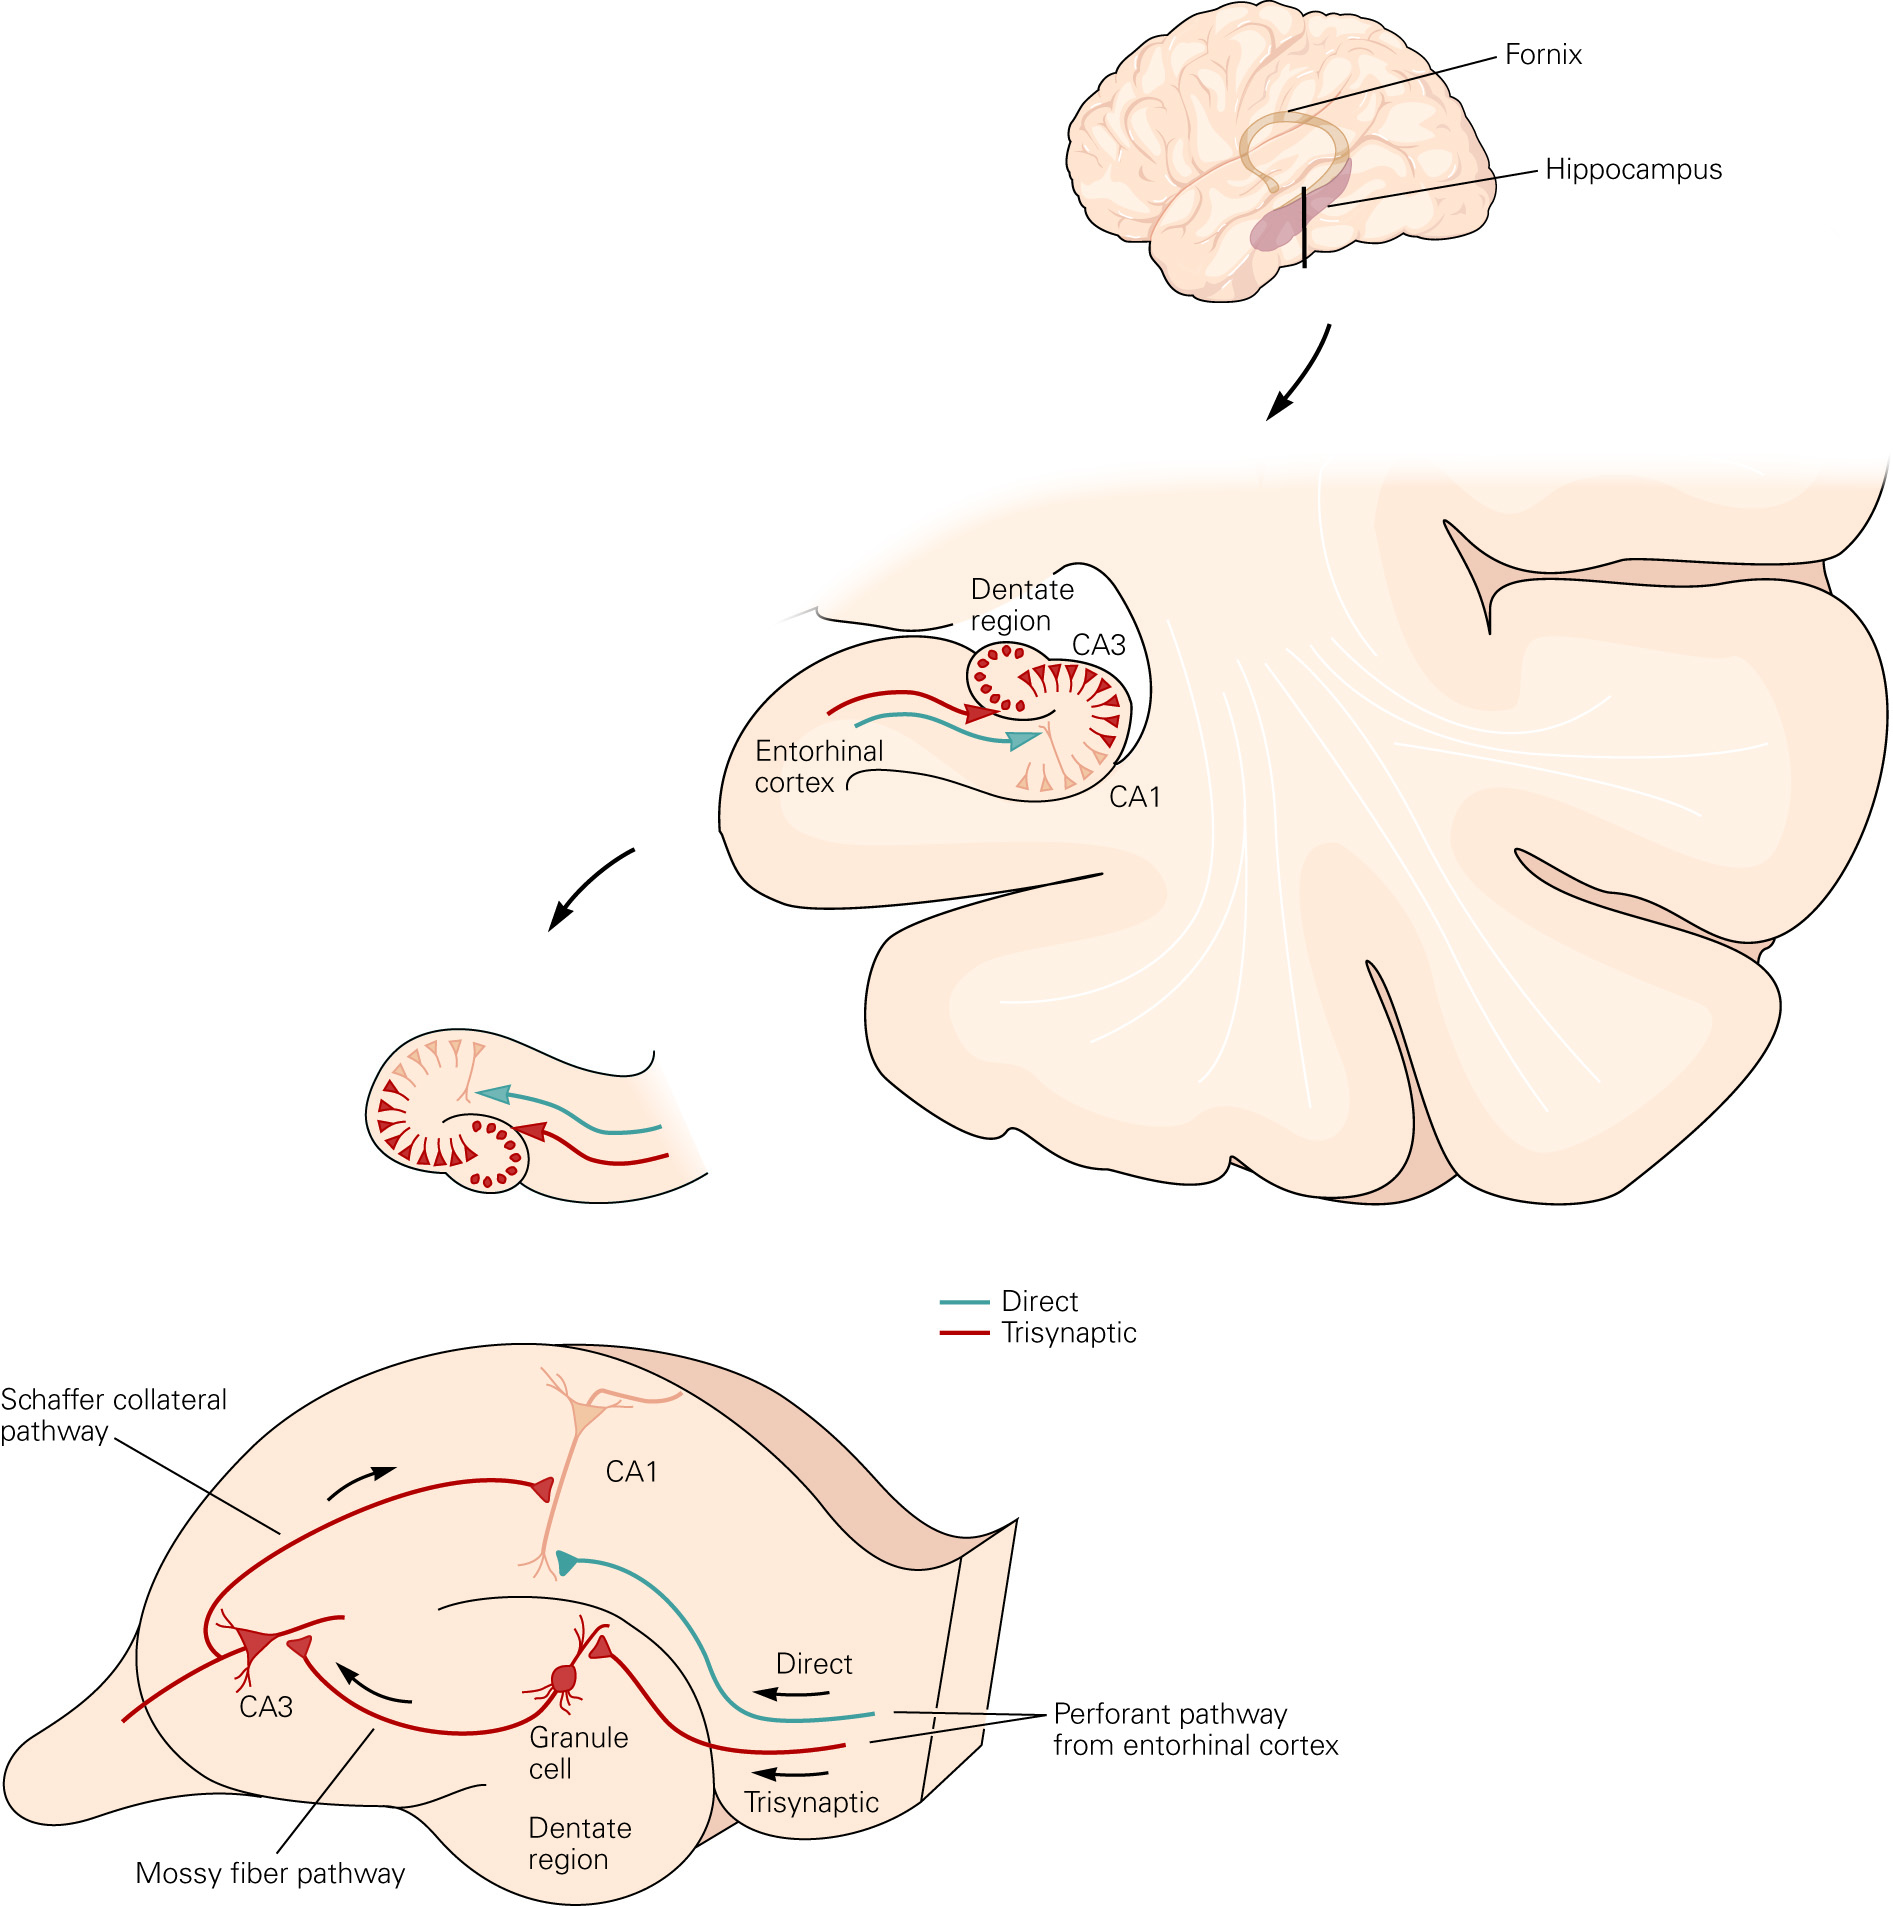
\includegraphics[scale=0.9]{Pic/6702_PNS5.jpg}
\end{figure}
CA1区域的椎体细胞通过不同的通路来获得信息输入这个事实让人们猜测:CA1区域的神经元会对这两个通路来的信息进行比较。动物损伤实验表明这两个通路对于学习和记忆来说缺一不可。研究表明在短期频繁的刺激下,直接通路和间接通路的第一个突触之间会生成LTP,这些LTP会持续几天到几周不等。而且相关研究表明,LTP并不是突触可塑性的单一形式,而是由多种加强海马区不同突触的突触传输过程的共同影响下形成的。这些过程涉及到各种不同的细胞及分子机制,甚至一个神经元能够引发多种LTP。但是,不同的LTP之间有很大的共性。共性在于LTP都需要突触后NMDA类型的谷氨酸受体,而差异性在于不同的NMDA类型的谷氨酸受体对于LTP的作用是不同的
\begin{figure}[h]
	\centering
	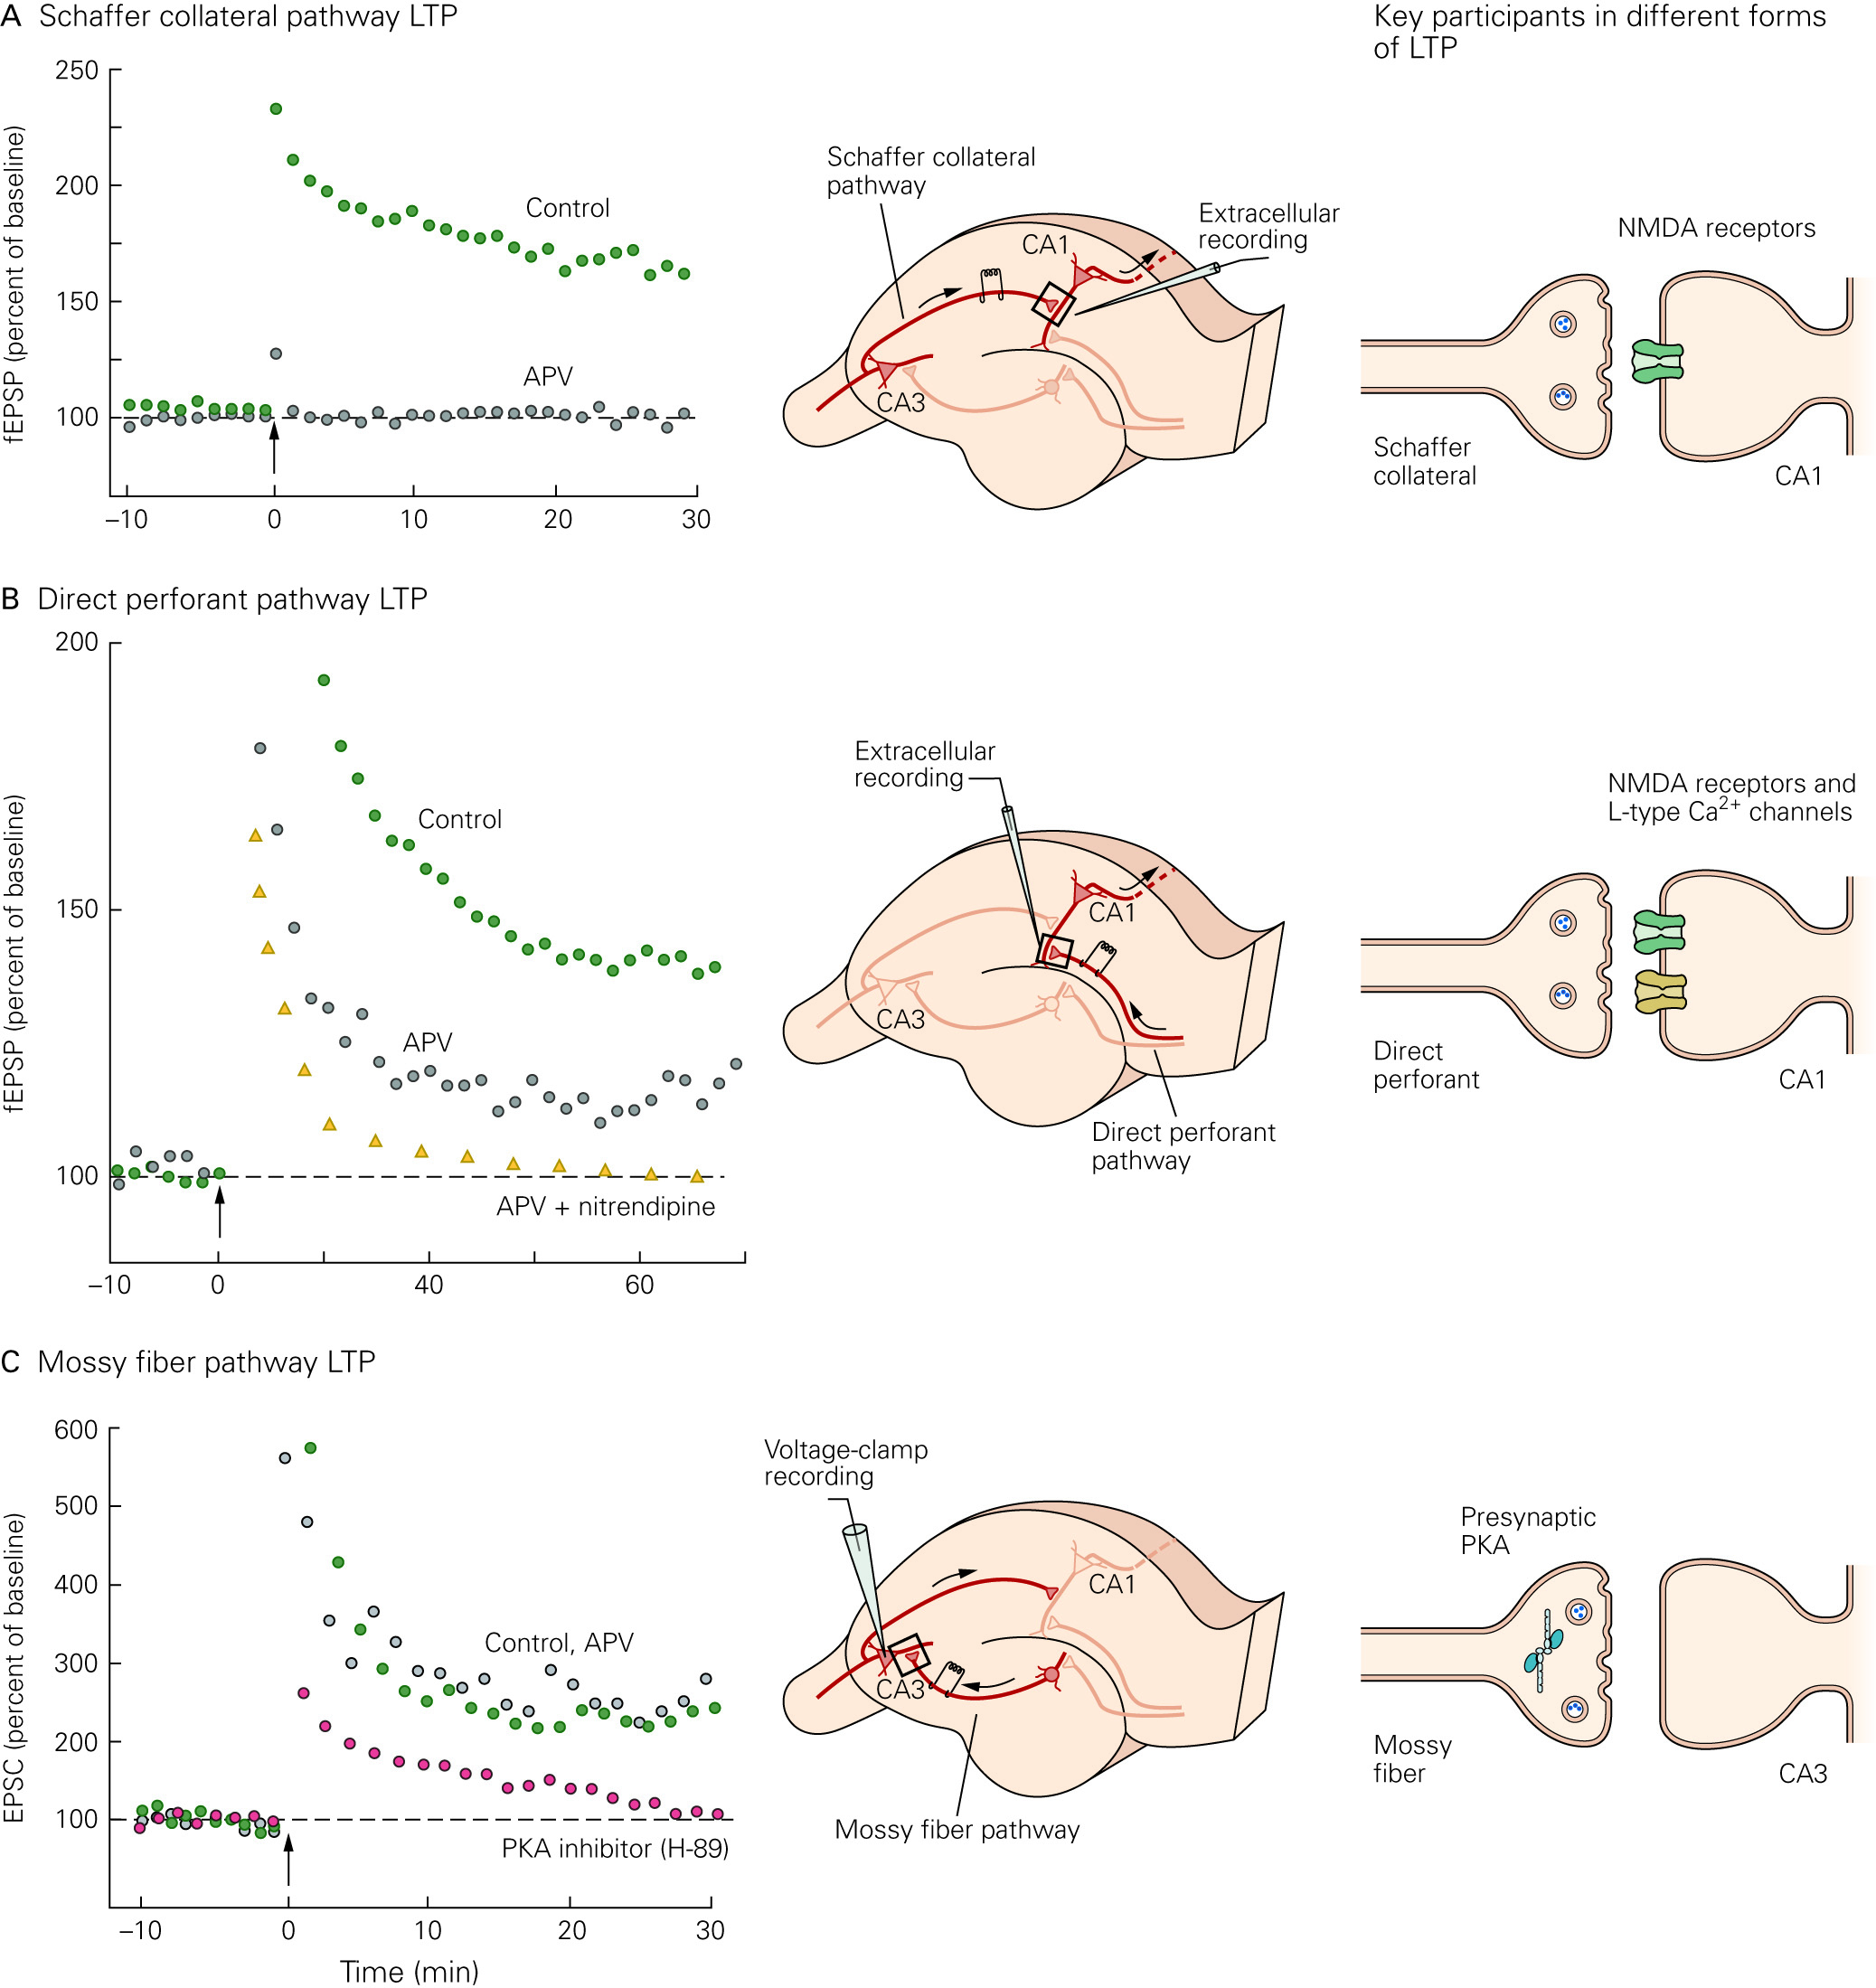
\includegraphics[scale=0.9]{Pic/6703_PNS5.jpg}
\end{figure}
LTP需要不同的二级信使来传递信号:要么通过在突触前细胞中起作用来改变突触的释放,要么在突触后起作用来改变受体对神经递质谷氨酸的敏感性。近期研究表明LTP的维持机制依赖于LTP的激发机制。在很多种情况下LTP是由于CA1突触后膜谷氨酸的NMDA受体活性增强所激发的钙离子内流所造成的。但是在一些情况下,LTP是由于突触前膜的递质释放易化所造成的。这里具体的机制就懒得说了,好复杂,不想翻译了。
\begin{figure}
	\centering
	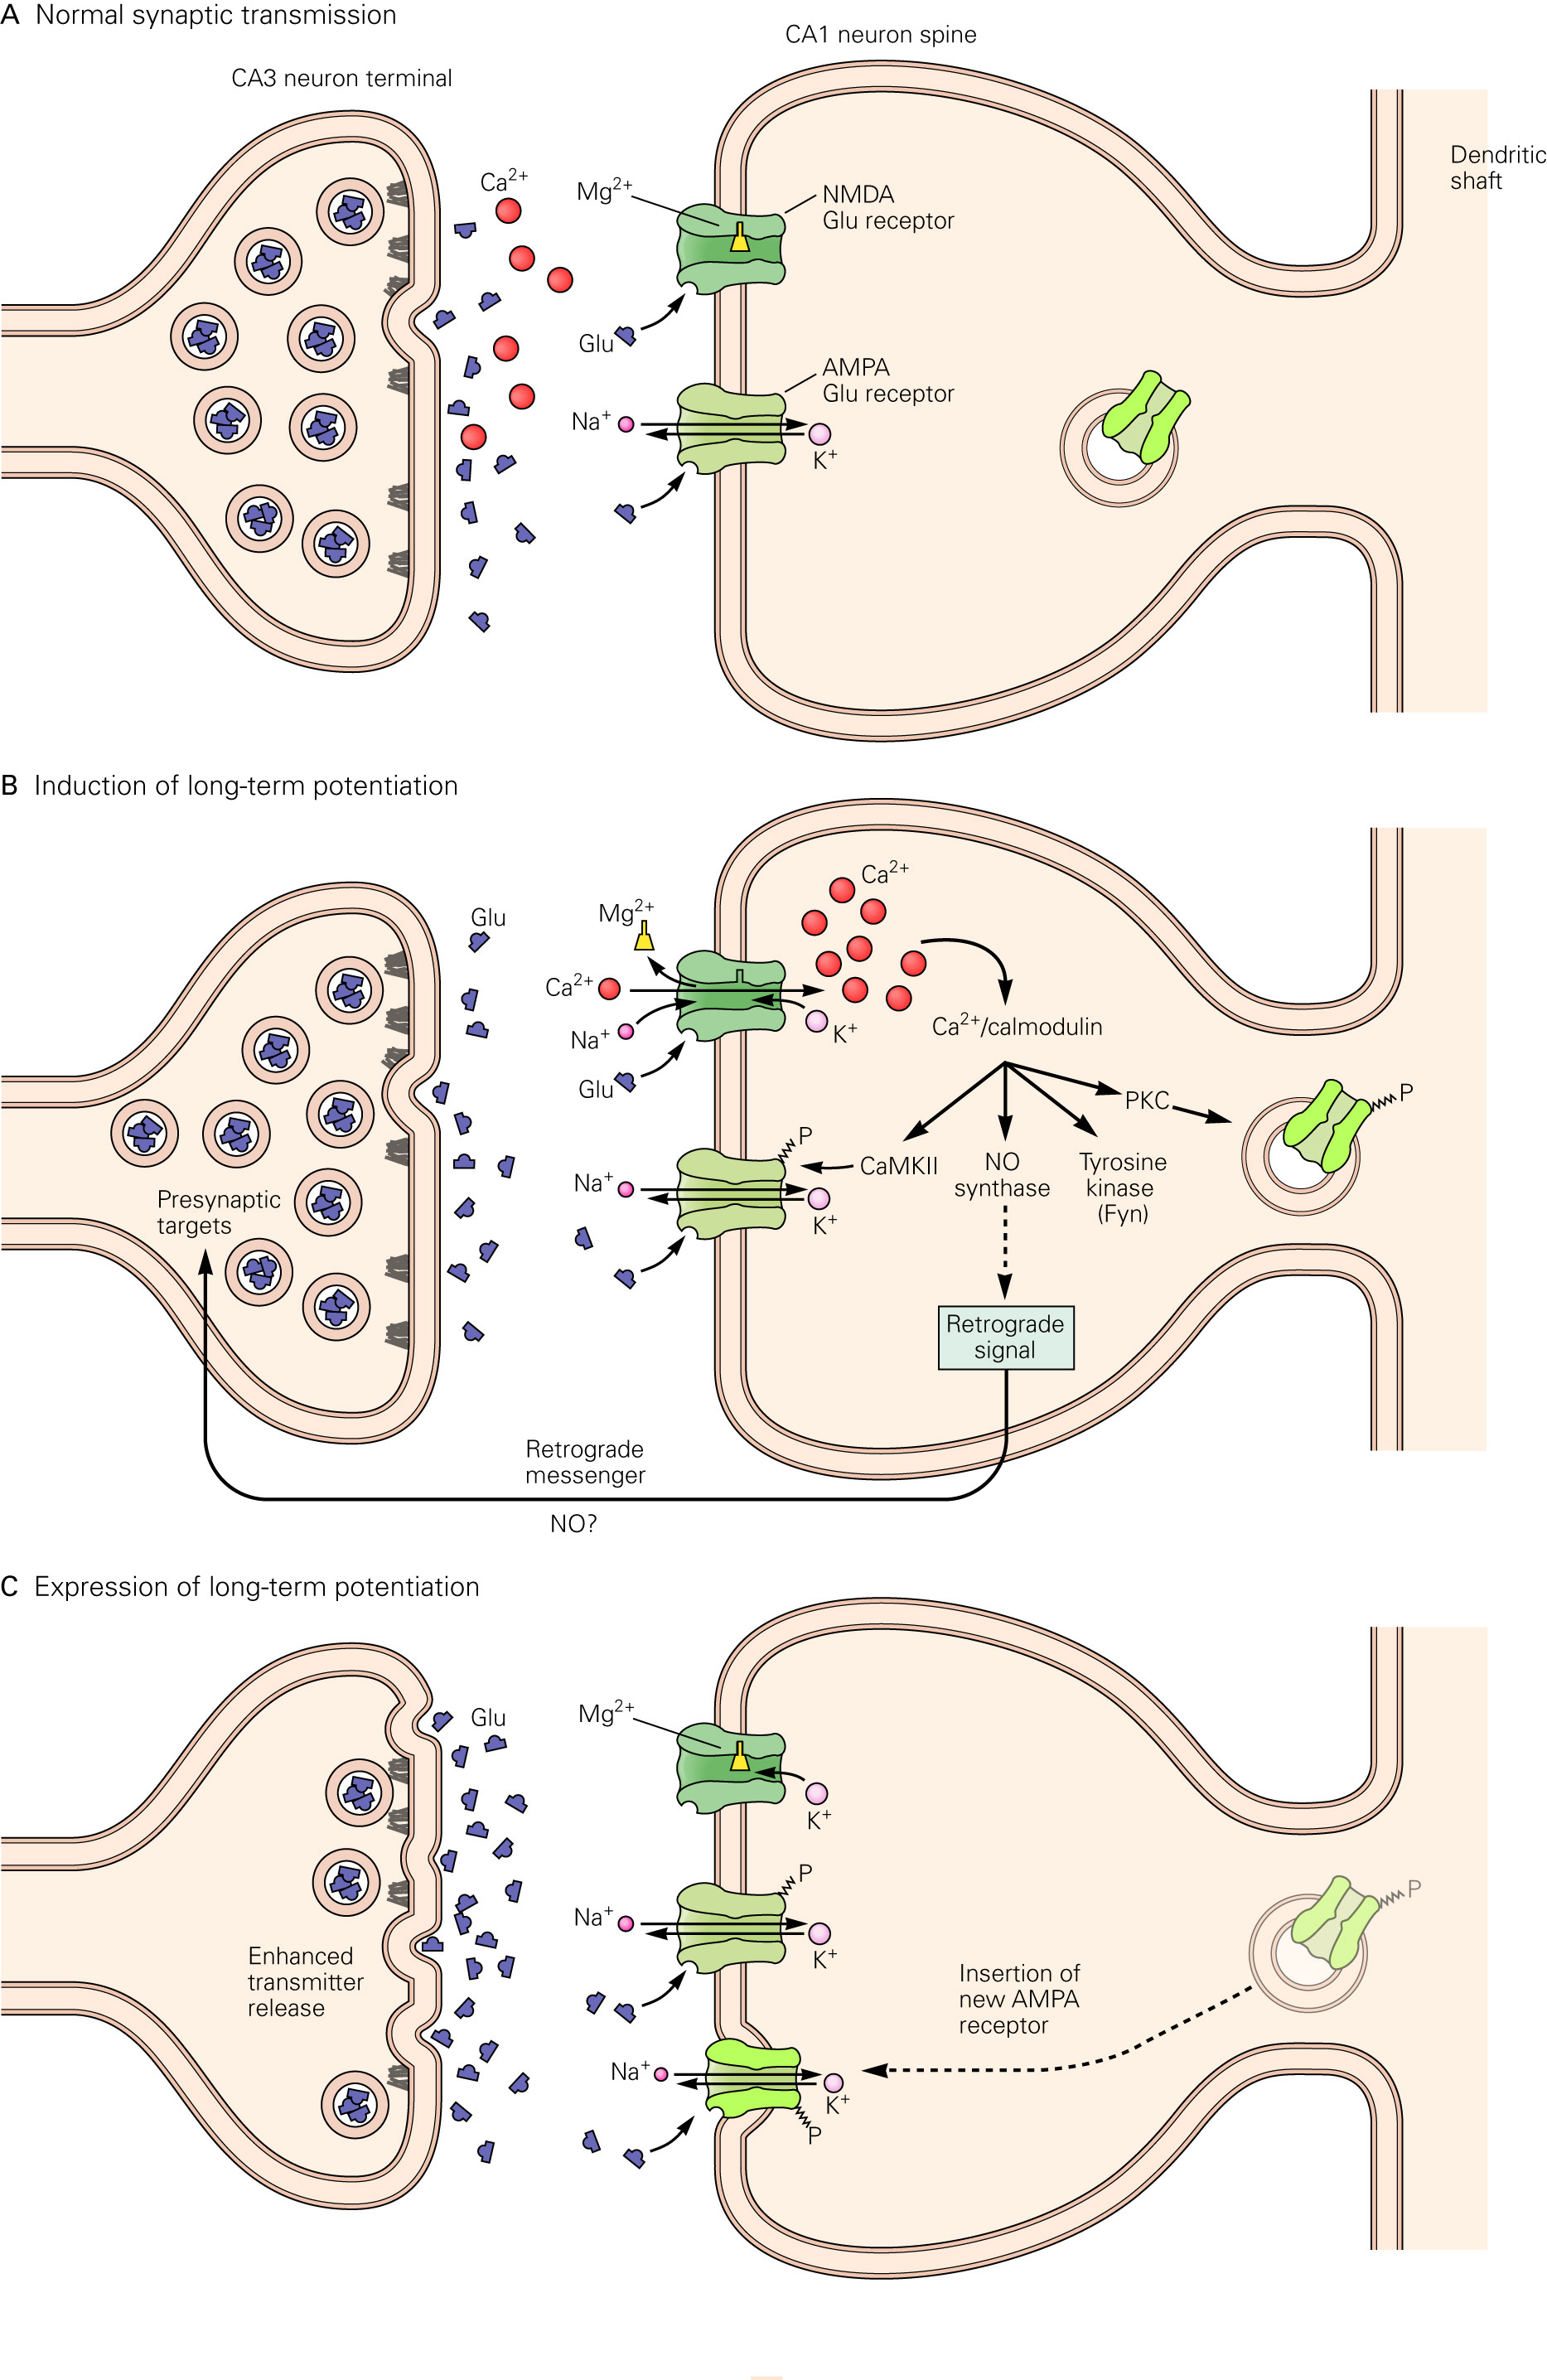
\includegraphics[scale=0.9]{Pic/6704_PNS5.jpg}
\end{figure}
\subsubsection{在schaffer collateral 通路中的LTP有hebbian 学习性质}
在Schaffer collateral通路中的NMDA受体赋予了LTP如下几个有趣的性质。
\begin{enumerate}
	\item 通路中的LTP需要附近一大波神经元的同步激活,也叫做copperativity。这个特性表现在为了减少镁离子对于NMDA的抑制作用需要一个大的去极化。
	\item  第二个有趣的特性叫做associativity。一个弱的刺激并不会引起足够的去极化来引发LTP。但是如果这个弱刺激伴随着一个强刺激的话,可以得到足够的去极化来引发LTP。
	\item 第三个特性是synaptic specific 。如果一个特定的突触并没有被一段强刺激所激活,则这个突触的NMDA受体则不能绑定谷氨酸,从而不能引发LTP。
\end{enumerate}
\begin{figure}[h]
	\centering
	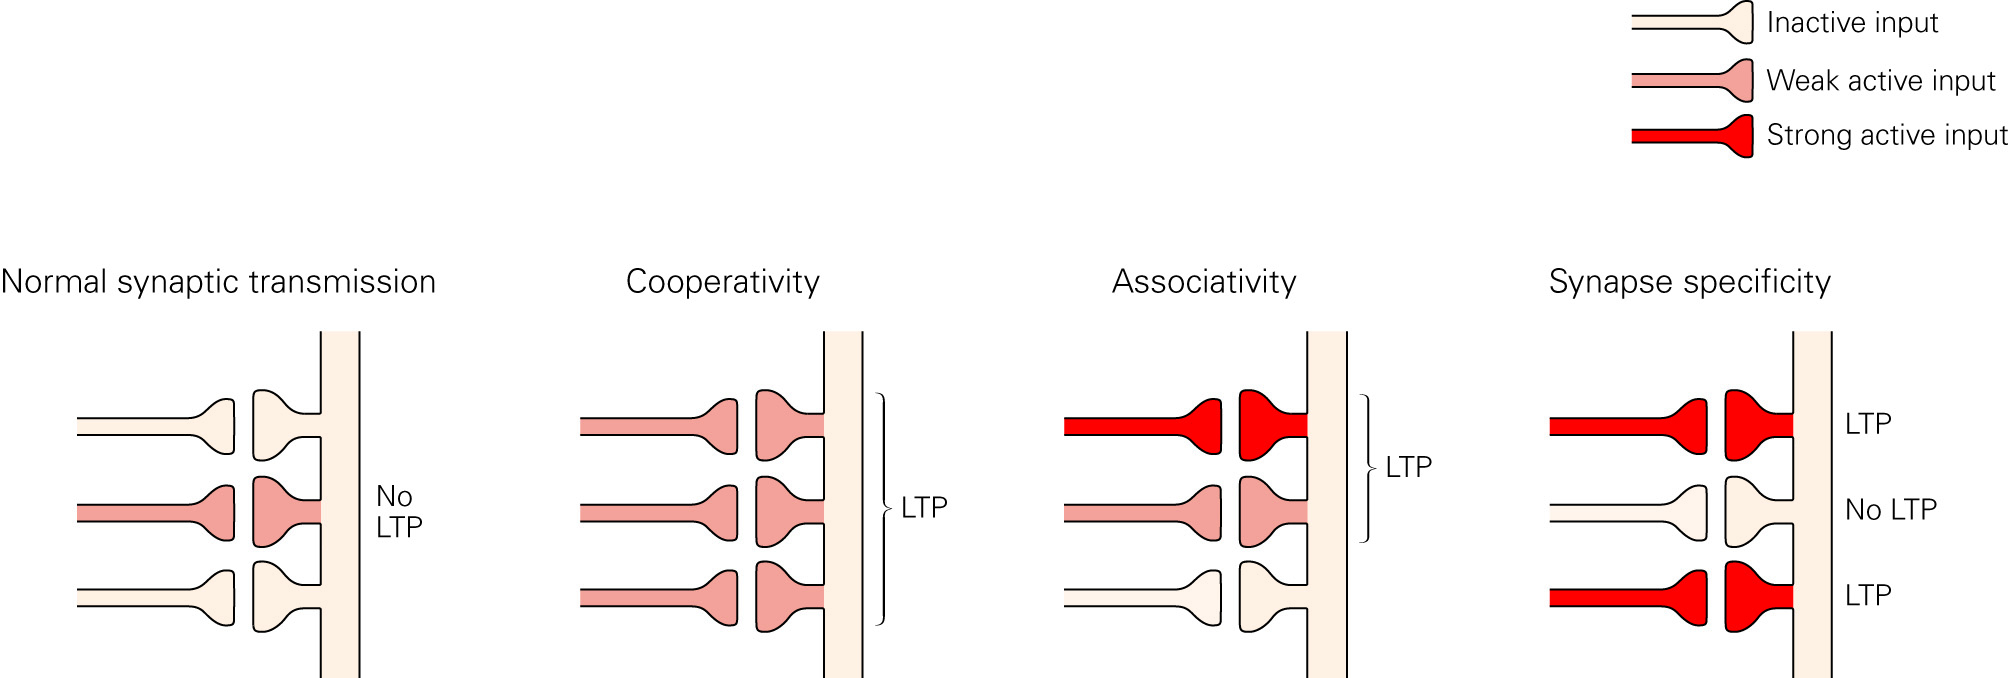
\includegraphics[scale=0.8]{Pic/6706_PNS5.jpg}
\end{figure}	
这三个性质刚好符合记忆的性质。Cooperativity保证只有那些很重要的事件(会引起多种输入)才会被记忆存储,Associativity就类似于巴普洛夫的铃铛实验,时间跨度很接近的输入信息也可转化为记忆。而synaptic specific则保证:如果一些输入所代表的信息与当前事件毫无联系,则这些信息的记忆则不会被当前事件所加强。
\par
所谓hebb's law 就是
\begin{quote}
	When an axon of cell A is near enough to excite a cell B and repeatedly or persistently takes part in firing it, some growth process or metabolic change takes place in one or both cells such that A's efficiency, as one of the cells firing B, is increased。
	\end{quote}
Schaffer collateral通路的LTP引发需要非常强烈的突触前活动这个发现给hebb's law提供了一些证据。LTP对于hebb's law 的解释在于刺激峰与突触可塑性之间的关系。大多数情况下,海马神经元并不会产生高频的电刺激,因此引发不了LTP。但是有一种LTP能够在突触前神经元和突触后神经元同时受刺激的情况下引发。当然条件非常严格,突触后刺激需要在突触前刺激的几ms之间引发,以产生类似高频的效果。在这个双重刺激下,镁离子对于NMDA的抑制作用会被减轻,从而导致钙离子内流并引发LTP。
\subsubsection{LTP有两种相:早期相和晚期相}
单次刺激能够引发LTP的早期相。LTP的早期相能够持续1-3个小时,并不需要新的蛋白质合成以及cAMP和PKA的激活。四次及以上的刺激能够依法长达24小时的LTP,这个晚期相的LTP需要cAMP和PKA,以及基因的表达。这里就懒得说了,有图为证。
\begin{figure}[h]
	\centering
	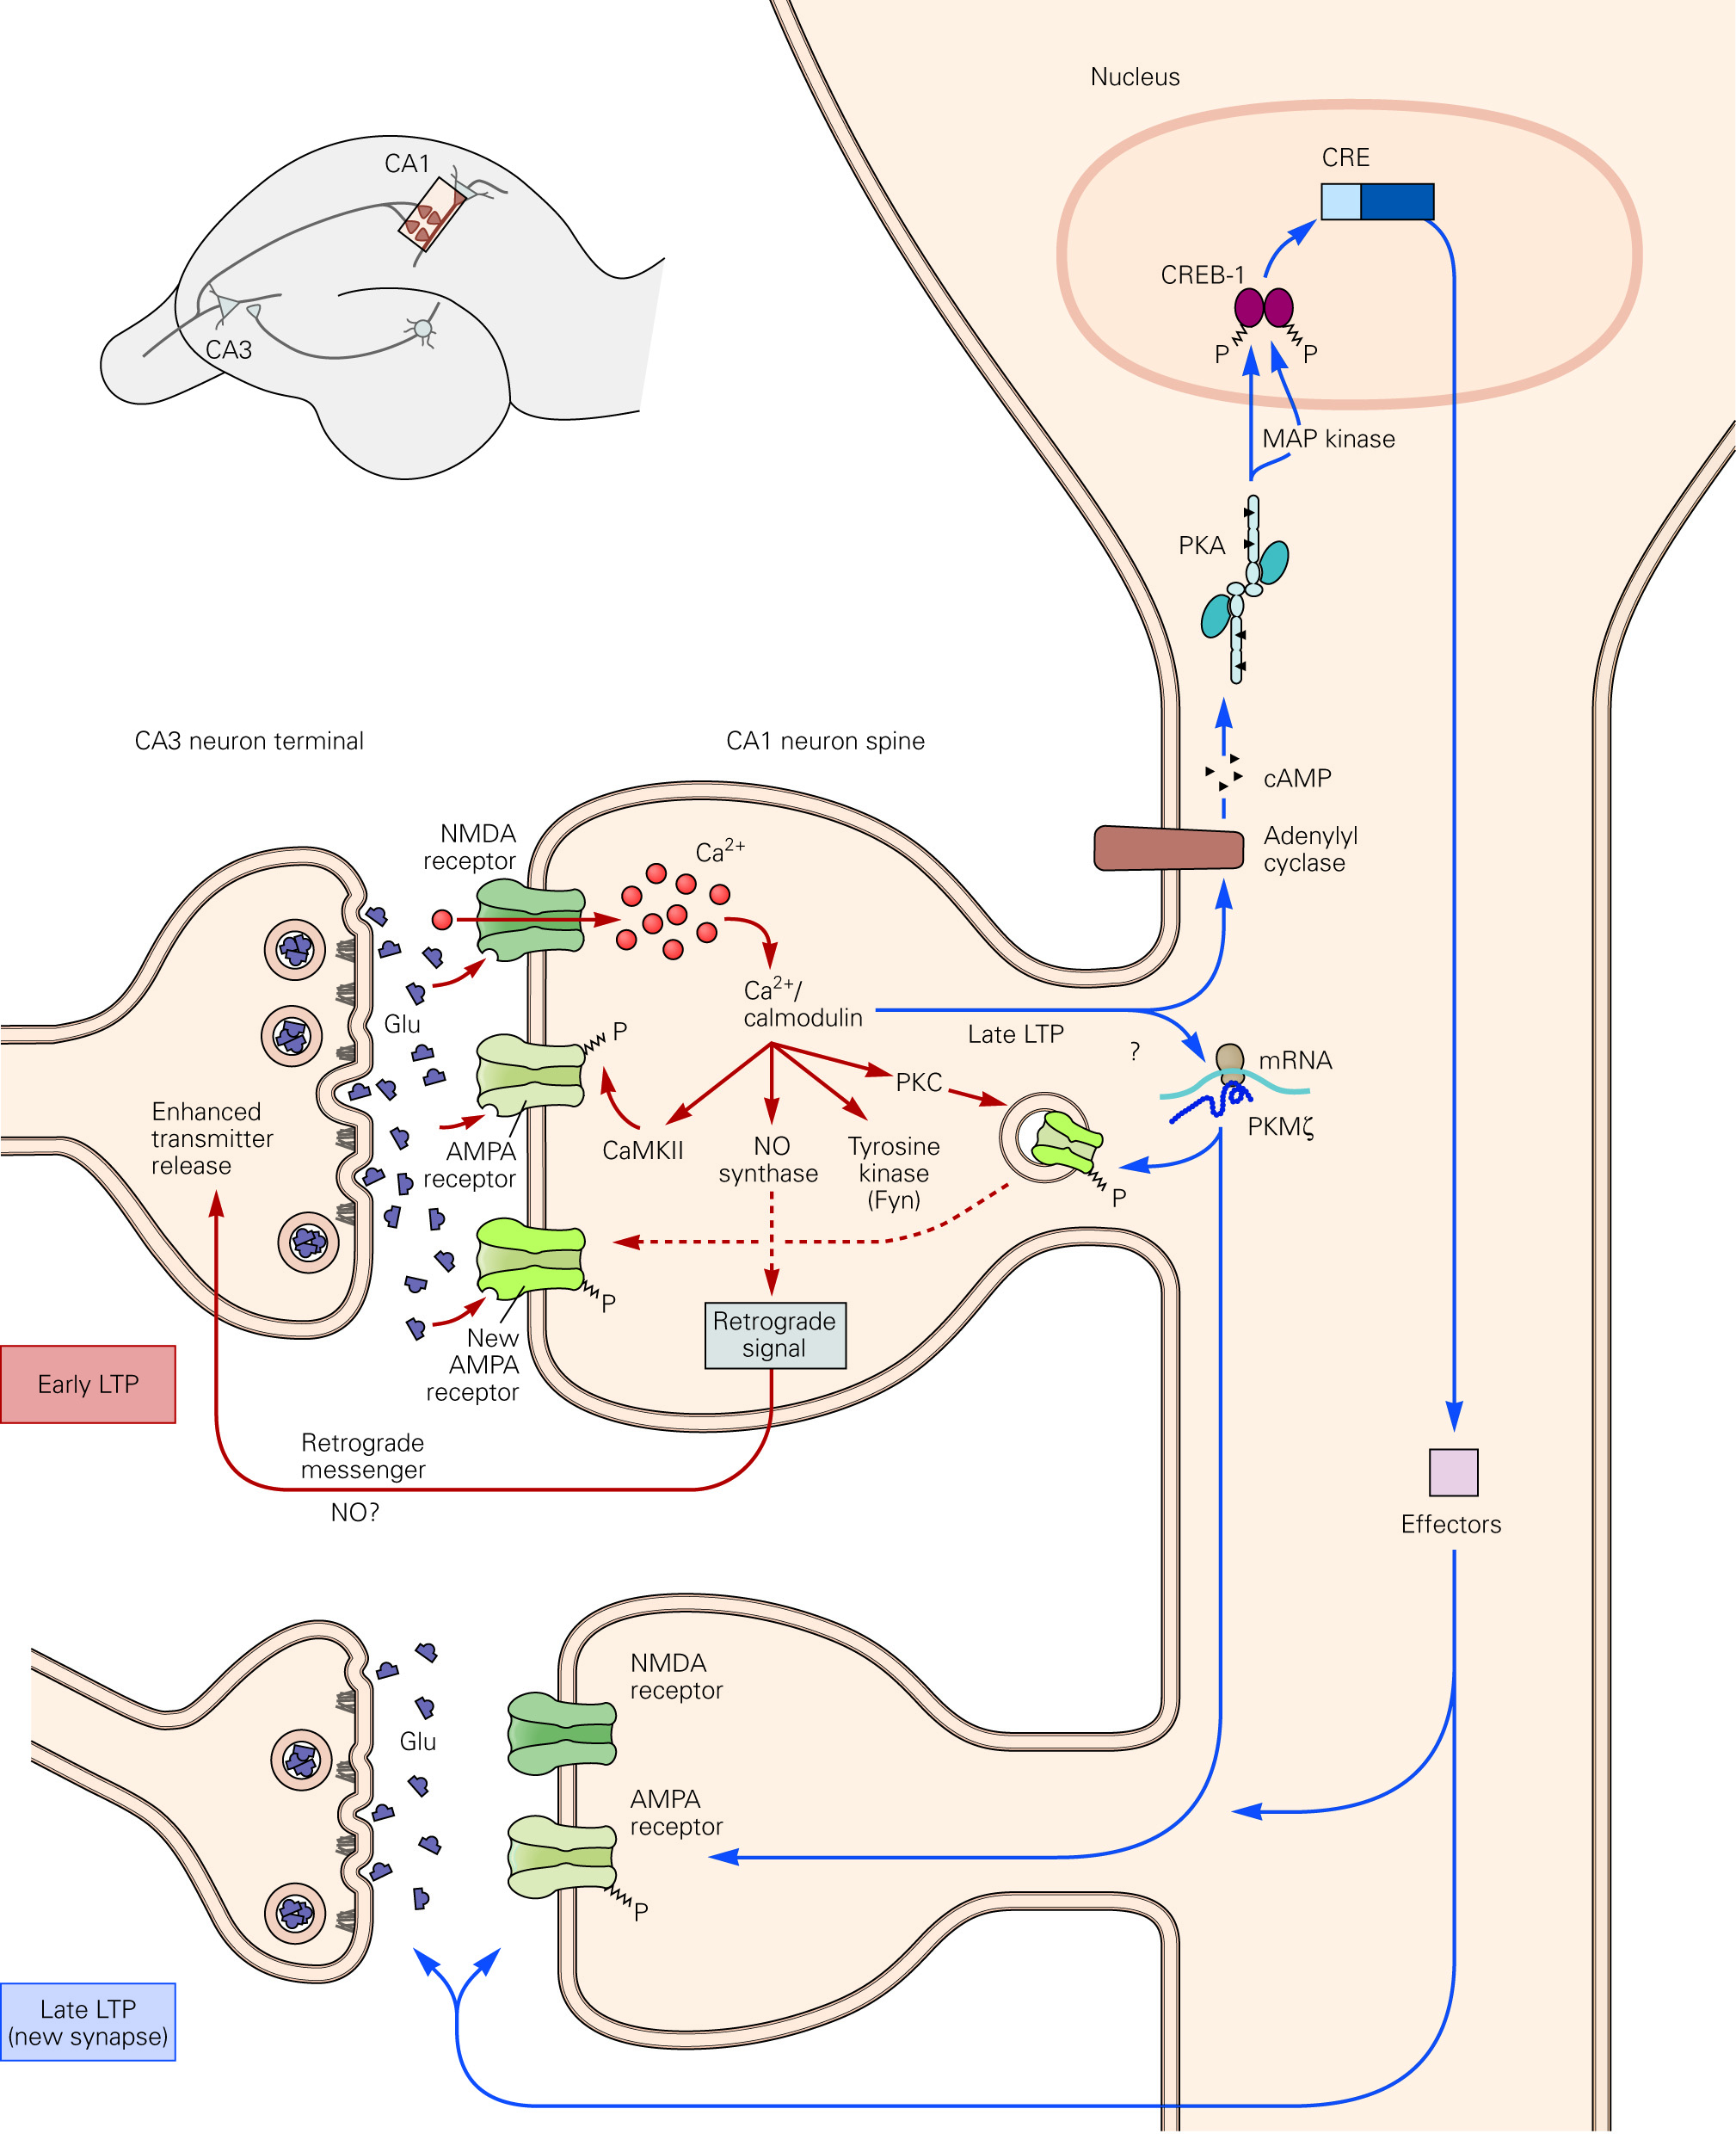
\includegraphics[scale=0.8]{Pic/6709_PNS5.jpg}
\end{figure}
\subsubsection{空间记忆依赖于海马的LTP}
目前很多实验都证明了抑制海马的LTP会影响到空间记忆,方法就是通过注入LTP的相关抑制剂之后进行老鼠走迷宫实验来观察空间记忆功能是否受损。常用的抑制剂有:NMDA抑制剂和PKM$\zeta$。NMDA对于早期LTP的生成起重要作用,而PKM$\zeta$对于长期LTP的维持有重要作用。用了NMDA抑制剂的后果就是什么都记不住,用了PKM$\zeta$的后果是现在记得住第二天就忘了。当然不仅仅可以用受体抑制剂来干扰LTP,还可以进行基因手段等手段来干涉LTP,要么敲除要么过表达。
\par
在逆向基因工程的帮助下,一种叫做CaMKII的酶被发现对于记忆的维持非常重要。这个酶在暴露在钙离子之后,会通过自动磷酸化苏氨酸-286(Thr286)转变为一种钙离子独立相。这种一经激活就能维持长期活性的性质使得人们认为CaMKII是一种记忆维持的分子开关。
\subsubsection{模式区分和模式补全牵涉到海马的不同区域}
显式记忆是用来存储事实(例如语义记忆)和场景记忆(例如昨天表白被拒)的。有效的记忆存储和检索需要大脑有区分相似图片、场景和空间的能力,这种能力叫做模式区分(pattern separation)。显式记忆也需要我们能够根据片段信息来获取之前存储的完整记忆的能力,这种能力叫做模式补全(pattern completion)。这两种能力对于高效的记忆系统都十分关键。
\par
早期的研究表明,模式补全依赖于CA3区域的椎体细胞的往返连接,而模式区分依赖于内嗅皮层到齿状沟回的直接投射。通过选择性的敲除NMDA谷氨酸受体基因,老鼠CA3区域往返神经连接引起的LTP受损,而mossy 纤维突触的LTP不受影响。
在这种实验条件下,老鼠在迷宫里面的学习能力并没有受到影响,然而,当转移到一个类似的迷宫时,老鼠的表现非常差。这个实验说明了CA3区域的往返连接对于模式补全来说非常重要。另外的一个实验通过选择性的敲除齿状沟回里的颗粒神经元NMDA谷氨酸受体的一个子单元,发现老鼠区分不同上下文的能力降低了。
\par
在神经科学中最意想不到的发现是神经形成并不仅限于生长发育的早期阶段,成年期也可以进行。但是成年期的神经形成只在两个脑区中进行:嗅球的抑制性颗粒细胞和齿状沟回中的激动性颗粒细胞。而且模式区分需要成年后新城的颗粒神经元的参与。
\subsubsection{记忆也需要突触传递的长期抑制}
总所周知,记忆是会退化的,因此一定会有某一种机制来拮抗LTP,暂且称之为LTD(Longterm depression)。LTD第一次在小脑中被发现,用来管理运动学习。之后在海马中也发现了LTD。不同于LTP是高频刺激所引发,LTD需要长期的类似于15分钟一次的低频刺激。令人惊奇的是,LTD跟LTP一样需要NMDA受体,也需要钙离子的内流。但是LTD所接受的低频刺激并不能够引发大强度的去极化,因此不能有效的减轻镁离子对于NMDA的抑制,所以钙离子内流量比较小。而低浓度的钙离子也无法激活CaMKII,所以LTD的过程应该是有一种比CaMKII对钙亲和性更高的钙调神经酶参与磷酸化过程。在此酶的作用下,引发AMPA受体的内吞,从而减少突触后膜的受体数量,并最终减少EPSP。更多的实验表明:LTD不仅仅对于阻止LTP的饱和有作用,还主动参与了记忆存储的过程。
\subsubsection{长期记忆也需要染色体的改变}
这里的染色体改变过程不仅仅在于CBP参与下的组蛋白改变,还有DNA的甲基化。这里的一些细节就不去细说了。

\par

\end{document}